\documentclass[journal]{IEEEtran}
%
% If IEEEtran.cls has not been installed into the LaTeX system files,
% manually specify the path to it like:
% \documentclass[journal]{../sty/IEEEtran}





% Some very useful LaTeX packages include:
% (uncomment the ones you want to load)
\usepackage[spanish]{babel}
\usepackage[utf8]{inputenc}
\usepackage{url}
\usepackage{minted}
\setminted{fontsize=\small,baselinestretch=1}
\usepackage{listings}
\usepackage{subcaption}
\renewcommand\listingscaption{Código}
\newenvironment{code}{\captionsetup{type=listing}}{\par\addvspace{\baselineskip}}
\usepackage{graphicx}
\usepackage{tikz}
\usetikzlibrary{scopes}
\usetikzlibrary{babel}
\usepackage{pgfplots}
\usepackage{amsmath}
\usepackage[americanvoltage]{circuitikz}


% *** MISC UTILITY PACKAGES ***
%
%\usepackage{ifpdf}
% Heiko Oberdiek's ifpdf.sty is very useful if you need conditional
% compilation based on whether the output is pdf or dvi.
% usage:
% \ifpdf
%   % pdf code
% \else
%   % dvi code
% \fi
% The latest version of ifpdf.sty can be obtained from:
% http://www.ctan.org/pkg/ifpdf
% Also, note that IEEEtran.cls V1.7 and later provides a builtin
% \ifCLASSINFOpdf conditional that works the same way.
% When switching from latex to pdflatex and vice-versa, the compiler may
% have to be run twice to clear warning/error messages.






% *** CITATION PACKAGES ***
%
%\usepackage{cite}
% cite.sty was written by Donald Arseneau
% V1.6 and later of IEEEtran pre-defines the format of the cite.sty package
% \cite{} output to follow that of the IEEE. Loading the cite package will
% result in citation numbers being automatically sorted and properly
% "compressed/ranged". e.g., [1], [9], [2], [7], [5], [6] without using
% cite.sty will become [1], [2], [5]--[7], [9] using cite.sty. cite.sty's
% \cite will automatically add leading space, if needed. Use cite.sty's
% noadjust option (cite.sty V3.8 and later) if you want to turn this off
% such as if a citation ever needs to be enclosed in parenthesis.
% cite.sty is already installed on most LaTeX systems. Be sure and use
% version 5.0 (2009-03-20) and later if using hyperref.sty.
% The latest version can be obtained at:
% http://www.ctan.org/pkg/cite
% The documentation is contained in the cite.sty file itself.






% *** GRAPHICS RELATED PACKAGES ***
%
\ifCLASSINFOpdf
  % \usepackage[pdftex]{graphicx}
  % declare the path(s) where your graphic files are
  % \graphicspath{{../pdf/}{../jpeg/}}
  % and their extensions so you won't have to specify these with
  % every instance of \includegraphics
  % \DeclareGraphicsExtensions{.pdf,.jpeg,.png}
\else
  % or other class option (dvipsone, dvipdf, if not using dvips). graphicx
  % will default to the driver specified in the system graphics.cfg if no
  % driver is specified.
  % \usepackage[dvips]{graphicx}
  % declare the path(s) where your graphic files are
  % \graphicspath{{../eps/}}
  % and their extensions so you won't have to specify these with
  % every instance of \includegraphics
  % \DeclareGraphicsExtensions{.eps}
\fi
% graphicx was written by David Carlisle and Sebastian Rahtz. It is
% required if you want graphics, photos, etc. graphicx.sty is already
% installed on most LaTeX systems. The latest version and documentation
% can be obtained at: 
% http://www.ctan.org/pkg/graphicx
% Another good source of documentation is "Using Imported Graphics in
% LaTeX2e" by Keith Reckdahl which can be found at:
% http://www.ctan.org/pkg/epslatex
%
% latex, and pdflatex in dvi mode, support graphics in encapsulated
% postscript (.eps) format. pdflatex in pdf mode supports graphics
% in .pdf, .jpeg, .png and .mps (metapost) formats. Users should ensure
% that all non-photo figures use a vector format (.eps, .pdf, .mps) and
% not a bitmapped formats (.jpeg, .png). The IEEE frowns on bitmapped formats
% which can result in "jaggedy"/blurry rendering of lines and letters as
% well as large increases in file sizes.
%
% You can find documentation about the pdfTeX application at:
% http://www.tug.org/applications/pdftex





% *** MATH PACKAGES ***
%
%\usepackage{amsmath}
% A popular package from the American Mathematical Society that provides
% many useful and powerful commands for dealing with mathematics.
%
% Note that the amsmath package sets \interdisplaylinepenalty to 10000
% thus preventing page breaks from occurring within multiline equations. Use:
%\interdisplaylinepenalty=2500
% after loading amsmath to restore such page breaks as IEEEtran.cls normally
% does. amsmath.sty is already installed on most LaTeX systems. The latest
% version and documentation can be obtained at:
% http://www.ctan.org/pkg/amsmath





% *** SPECIALIZED LIST PACKAGES ***
%
%\usepackage{algorithmic}
% algorithmic.sty was written by Peter Williams and Rogerio Brito.
% This package provides an algorithmic environment fo describing algorithms.
% You can use the algorithmic environment in-text or within a figure
% environment to provide for a floating algorithm. Do NOT use the algorithm
% floating environment provided by algorithm.sty (by the same authors) or
% algorithm2e.sty (by Christophe Fiorio) as the IEEE does not use dedicated
% algorithm float types and packages that provide these will not provide
% correct IEEE style captions. The latest version and documentation of
% algorithmic.sty can be obtained at:
% http://www.ctan.org/pkg/algorithms
% Also of interest may be the (relatively newer and more customizable)
% algorithmicx.sty package by Szasz Janos:
% http://www.ctan.org/pkg/algorithmicx




% *** ALIGNMENT PACKAGES ***
%
%\usepackage{array}
% Frank Mittelbach's and David Carlisle's array.sty patches and improves
% the standard LaTeX2e array and tabular environments to provide better
% appearance and additional user controls. As the default LaTeX2e table
% generation code is lacking to the point of almost being broken with
% respect to the quality of the end results, all users are strongly
% advised to use an enhanced (at the very least that provided by array.sty)
% set of table tools. array.sty is already installed on most systems. The
% latest version and documentation can be obtained at:
% http://www.ctan.org/pkg/array


% IEEEtran contains the IEEEeqnarray family of commands that can be used to
% generate multiline equations as well as matrices, tables, etc., of high
% quality.




% *** SUBFIGURE PACKAGES ***
%\ifCLASSOPTIONcompsoc
%  \usepackage[caption=false,font=normalsize,labelfont=sf,textfont=sf]{subfig}
%\else
%  \usepackage[caption=false,font=footnotesize]{subfig}
%\fi
% subfig.sty, written by Steven Douglas Cochran, is the modern replacement
% for subfigure.sty, the latter of which is no longer maintained and is
% incompatible with some LaTeX packages including fixltx2e. However,
% subfig.sty requires and automatically loads Axel Sommerfeldt's caption.sty
% which will override IEEEtran.cls' handling of captions and this will result
% in non-IEEE style figure/table captions. To prevent this problem, be sure
% and invoke subfig.sty's "caption=false" package option (available since
% subfig.sty version 1.3, 2005/06/28) as this is will preserve IEEEtran.cls
% handling of captions.
% Note that the Computer Society format requires a larger sans serif font
% than the serif footnote size font used in traditional IEEE formatting
% and thus the need to invoke different subfig.sty package options depending
% on whether compsoc mode has been enabled.
%
% The latest version and documentation of subfig.sty can be obtained at:
% http://www.ctan.org/pkg/subfig




% *** FLOAT PACKAGES ***
%
%\usepackage{fixltx2e}
% fixltx2e, the successor to the earlier fix2col.sty, was written by
% Frank Mittelbach and David Carlisle. This package corrects a few problems
% in the LaTeX2e kernel, the most notable of which is that in current
% LaTeX2e releases, the ordering of single and double column floats is not
% guaranteed to be preserved. Thus, an unpatched LaTeX2e can allow a
% single column figure to be placed prior to an earlier double column
% figure.
% Be aware that LaTeX2e kernels dated 2015 and later have fixltx2e.sty's
% corrections already built into the system in which case a warning will
% be issued if an attempt is made to load fixltx2e.sty as it is no longer
% needed.
% The latest version and documentation can be found at:
% http://www.ctan.org/pkg/fixltx2e


%\usepackage{stfloats}
% stfloats.sty was written by Sigitas Tolusis. This package gives LaTeX2e
% the ability to do double column floats at the bottom of the page as well
% as the top. (e.g., "\begin{figure*}[!b]" is not normally possible in
% LaTeX2e). It also provides a command:
%\fnbelowfloat
% to enable the placement of footnotes below bottom floats (the standard
% LaTeX2e kernel puts them above bottom floats). This is an invasive package
% which rewrites many portions of the LaTeX2e float routines. It may not work
% with other packages that modify the LaTeX2e float routines. The latest
% version and documentation can be obtained at:
% http://www.ctan.org/pkg/stfloats
% Do not use the stfloats baselinefloat ability as the IEEE does not allow
% \baselineskip to stretch. Authors submitting work to the IEEE should note
% that the IEEE rarely uses double column equations and that authors should try
% to avoid such use. Do not be tempted to use the cuted.sty or midfloat.sty
% packages (also by Sigitas Tolusis) as the IEEE does not format its papers in
% such ways.
% Do not attempt to use stfloats with fixltx2e as they are incompatible.
% Instead, use Morten Hogholm'a dblfloatfix which combines the features
% of both fixltx2e and stfloats:
%
% \usepackage{dblfloatfix}
% The latest version can be found at:
% http://www.ctan.org/pkg/dblfloatfix




%\ifCLASSOPTIONcaptionsoff
%  \usepackage[nomarkers]{endfloat}
% \let\MYoriglatexcaption\caption
% \renewcommand{\caption}[2][\relax]{\MYoriglatexcaption[#2]{#2}}
%\fi
% endfloat.sty was written by James Darrell McCauley, Jeff Goldberg and 
% Axel Sommerfeldt. This package may be useful when used in conjunction with 
% IEEEtran.cls'  captionsoff option. Some IEEE journals/societies require that
% submissions have lists of figures/tables at the end of the paper and that
% figures/tables without any captions are placed on a page by themselves at
% the end of the document. If needed, the draftcls IEEEtran class option or
% \CLASSINPUTbaselinestretch interface can be used to increase the line
% spacing as well. Be sure and use the nomarkers option of endfloat to
% prevent endfloat from "marking" where the figures would have been placed
% in the text. The two hack lines of code above are a slight modification of
% that suggested by in the endfloat docs (section 8.4.1) to ensure that
% the full captions always appear in the list of figures/tables - even if
% the user used the short optional argument of \caption[]{}.
% IEEE papers do not typically make use of \caption[]'s optional argument,
% so this should not be an issue. A similar trick can be used to disable
% captions of packages such as subfig.sty that lack options to turn off
% the subcaptions:
% For subfig.sty:
% \let\MYorigsubfloat\subfloat
% \renewcommand{\subfloat}[2][\relax]{\MYorigsubfloat[]{#2}}
% However, the above trick will not work if both optional arguments of
% the \subfloat command are used. Furthermore, there needs to be a
% description of each subfigure *somewhere* and endfloat does not add
% subfigure captions to its list of figures. Thus, the best approach is to
% avoid the use of subfigure captions (many IEEE journals avoid them anyway)
% and instead reference/explain all the subfigures within the main caption.
% The latest version of endfloat.sty and its documentation can obtained at:
% http://www.ctan.org/pkg/endfloat
%
% The IEEEtran \ifCLASSOPTIONcaptionsoff conditional can also be used
% later in the document, say, to conditionally put the References on a 
% page by themselves.

% *** PDF, URL AND HYPERLINK PACKAGES ***
%
%\usepackage{url}
% url.sty was written by Donald Arseneau. It provides better support for
% handling and breaking URLs. url.sty is already installed on most LaTeX
% systems. The latest version and documentation can be obtained at:
% http://www.ctan.org/pkg/url
% Basically, \url{my_url_here}.


% *** Do not adjust lengths that control margins, column widths, etc. ***
% *** Do not use packages that alter fonts (such as pslatex).         ***
% There should be no need to do such things with IEEEtran.cls V1.6 and later.
% (Unless specifically asked to do so by the journal or conference you plan
% to submit to, of course. )


% correct bad hyphenation here
\hyphenation{op-tical net-works semi-conduc-tor}


\begin{document}
%
% paper title
% Titles are generally capitalized except for words such as a, an, and, as,
% at, but, by, for, in, nor, of, on, or, the, to and up, which are usually
% not capitalized unless they are the first or last word of the title.
% Linebreaks \\ can be used within to get better formatting as desired.
% Do not put math or special symbols in the title.
\title{Circuitos de Corriente Alterna}
%
%
% author names and IEEE memberships
% note positions of commas and nonbreaking spaces ( ~ ) LaTeX will not break
% a structure at a ~ so this keeps an author's name from being broken across
% two lines.
% use \thanks{} to gain access to the first footnote area
% a separate \thanks must be used for each paragraph as LaTeX2e's \thanks
% was not built to handle multiple paragraphs
%

\author{Alberto García García\\ (48718198-N)\\ \texttt{agg180@alu.ua.es} % <-this % stops a space
\thanks{}%
}


% The paper headers
\markboth{Física II -- Grado en Física -- 2018-2019}%
{}
% The only time the second header will appear is for the odd numbered pages
% after the title page when using the twoside option.
% 
% *** Note that you probably will NOT want to include the author's ***
% *** name in the headers of peer review papers.                   ***
% You can use \ifCLASSOPTIONpeerreview for conditional compilation here if
% you desire.


% make the title area
\maketitle

% As a general rule, do not put math, special symbols or citations
% in the abstract or keywords.
\begin{abstract}
En esta segunda práctica de la asignatura Física II del Grado en Física (curso académico 2018-2019) estudiaremos la dinámica de circuitos RLC (resistencia, bobina, condensador). Para ello, analizaremos dos casos distintos: en el primero de ellos veremos la descarga de un condensador inicialmente cargado en el que no existe un generador; en el segundo el circuito contará con un generador de corriente alterna. Para el primero de ellos estudiaremos tres situaciones distintas dependiendo de la resistencia: subamortiguación, amortiguación y sobreamortiguación; también calcularemos la energía total disipada en la resistencia. Por otro lado, en el segundo caso llevaremos a cabo un estudio teórico mediante el método de los fasores (que confirmaremos con la simulación) y por último realizaremos un estudio de resonancia.

El código Python que implementa esta práctica así las modificaciones realizadas a sus rutinas de visualización y las fuentes \LaTeX de este informe se encuentran disponibles online en el repositorio \url{https://github.com/Blitzman/physics/tree/master/fisica_2/practica_2}.
\end{abstract}


% For peer review papers, you can put extra information on the cover
% page as needed:
% \ifCLASSOPTIONpeerreview
% \begin{center} \bfseries EDICS Category: 3-BBND \end{center}
% \fi
%
% For peerreview papers, this IEEEtran command inserts a page break and
% creates the second title. It will be ignored for other modes.
\IEEEpeerreviewmaketitle

\section{Introducción}

\IEEEPARstart{E}{n} esta práctica estudiaremos mediante el uso de programas en el lenguaje Python la dinámica de circuitos RLC tanto con generador como sin él. Para ello, resolveremos las ecuaciones diferenciales que regulan dicha dinámica mediante el uso de algoritmos. Así pues, en la Sección \ref{sec:rlcnogenerador} estudiaremos el caso sin generador mientras que en la Sección \ref{sec:rlccongenerador} abordaremos la situación con generador.

\section{Circuito RLC en Serie sin Generador}
\label{sec:rlcnogenerador}

El sistema que estudiaremos en esta primera sección es el mostrado en la Figura \ref{fig:rlc}. En este caso disponemos de: un condensador inicialmente cargado $C$, una resistencia $R$, una bobina $L$ y un interruptor abierto. A tiempo cero se cierra el interruptor y se estudia cómo evoluciona el sistema.

\begin{figure}[!htb]
    \centering
    \begin{circuitikz}
        \draw[ very thick](5,3)-- +(30:0.46);
        \draw (0,0)
          to[C=\(C\),i=$I$] (0,3) % The voltage source
          to[R=\(R\),i=$I$] (5,3) % The resistor
          to[short,-o](5,3)
          (5.5,3)to[short,o-](6,3)
          to[L=\(L\),i=$I$] (6,0) % The inductor
          to (0,0); %Inductor One
        \end{circuitikz}
        \medskip
        \caption{Circuito RLC en serie sin generador.}
        \label{fig:rlc}
\end{figure}

De forma teórica, podemos afirmar que la carga $Q$ del condensador obedece a la siguiente ecuación diferencial:

\begin{equation}
L\frac{d^2Q}{dt} + R\frac{dQ}{dt} + \frac{Q}{C} = 0 ~,
\end{equation}

siendo esta ecuación totalmente análoga a la de un oscilador armónico amortiguado y que presenta las mismas soluciones. En el caso de la práctica, el programa \mintinline{c}{RCL.py} hace uso de la rutina \mintinline{c}{odeint} para resolver dicha ecuación diferencial para tres casos diferentes: amortiguado, subamortiguado y sobreamortiguado.

La frecuencia de oscilación en cada uno de los casos se puede calcular como:

\begin{equation}
f = \frac{1}{2\pi\sqrt{LC}}~[Hz]
\end{equation}

A continuación analizaremos la dinámica de dichos circuitos en los tres casos usando el programa de integración proporcionado. Para ello emplearemos los siguientes valores para el condensador $C~[F]$, la bobina $L~[H]$ y el tiempo de simulación tal como se muestra en el Código \ref{listing:datos_rlc}.

\bigskip

\begin{code}
    \begin{minted}{python}
        C=75.0e-6  # Condensador
        L=0.15 # Bobina
        tf=1.0e-1 # Tiempo de simulación
    \end{minted}
    \caption{Datos de simulación para estudio de dinámica de circuito RLC sin generador.}
    \label{listing:datos_rlc}
\end{code}

Por otro lado, la resistencia $R$ tendrá valores diferentes dependiendo de si el caso es amortiguado ($R=0~[\Omega]$), subamortiguado ($R^2 < 4L/C ~ [\Omega]$) y sobreamortiguado ($R^2 > 4L/C ~ [\Omega]$).

Para todos los casos representaremos la carga y la intensidad en función del tiempo $Q = f(t)~[C]$ e $I = (f)~[A]$ respectivamente. Además, también representaremos la variación de la energía magnética $U_m~[J]$, la energía electrostática $U_e~[J]$ y la suma de las dos $U~[J]$.

También comprobaremos, a partir de las gráficas planteadas, que la frecuencia de oscilación teórica anteriormente expuesta coincide con la frecuencia de oscilación de las mismas.

\subsection{Oscilador Amortiguado}
\label{subsec:osciladoramortiguado}

En esta sección estudiaremos el caso amortiguado, para el cual hemos elegido una resistencia de $R=0~[\Omega]$ y hemos ejecutado el programa \mintinline{c}{RLC.py} modificado para obtener las gráficas de evolución de la carga (ver Figura \ref{fig:cargaamortiguado}), de la intensidad (Figura \ref{fig:intensidadamortiguado}) y de las energías (Figura \ref{fig:energiaamortiguado}).

\newpage

\begin{figure}[!htb]
    \centering
    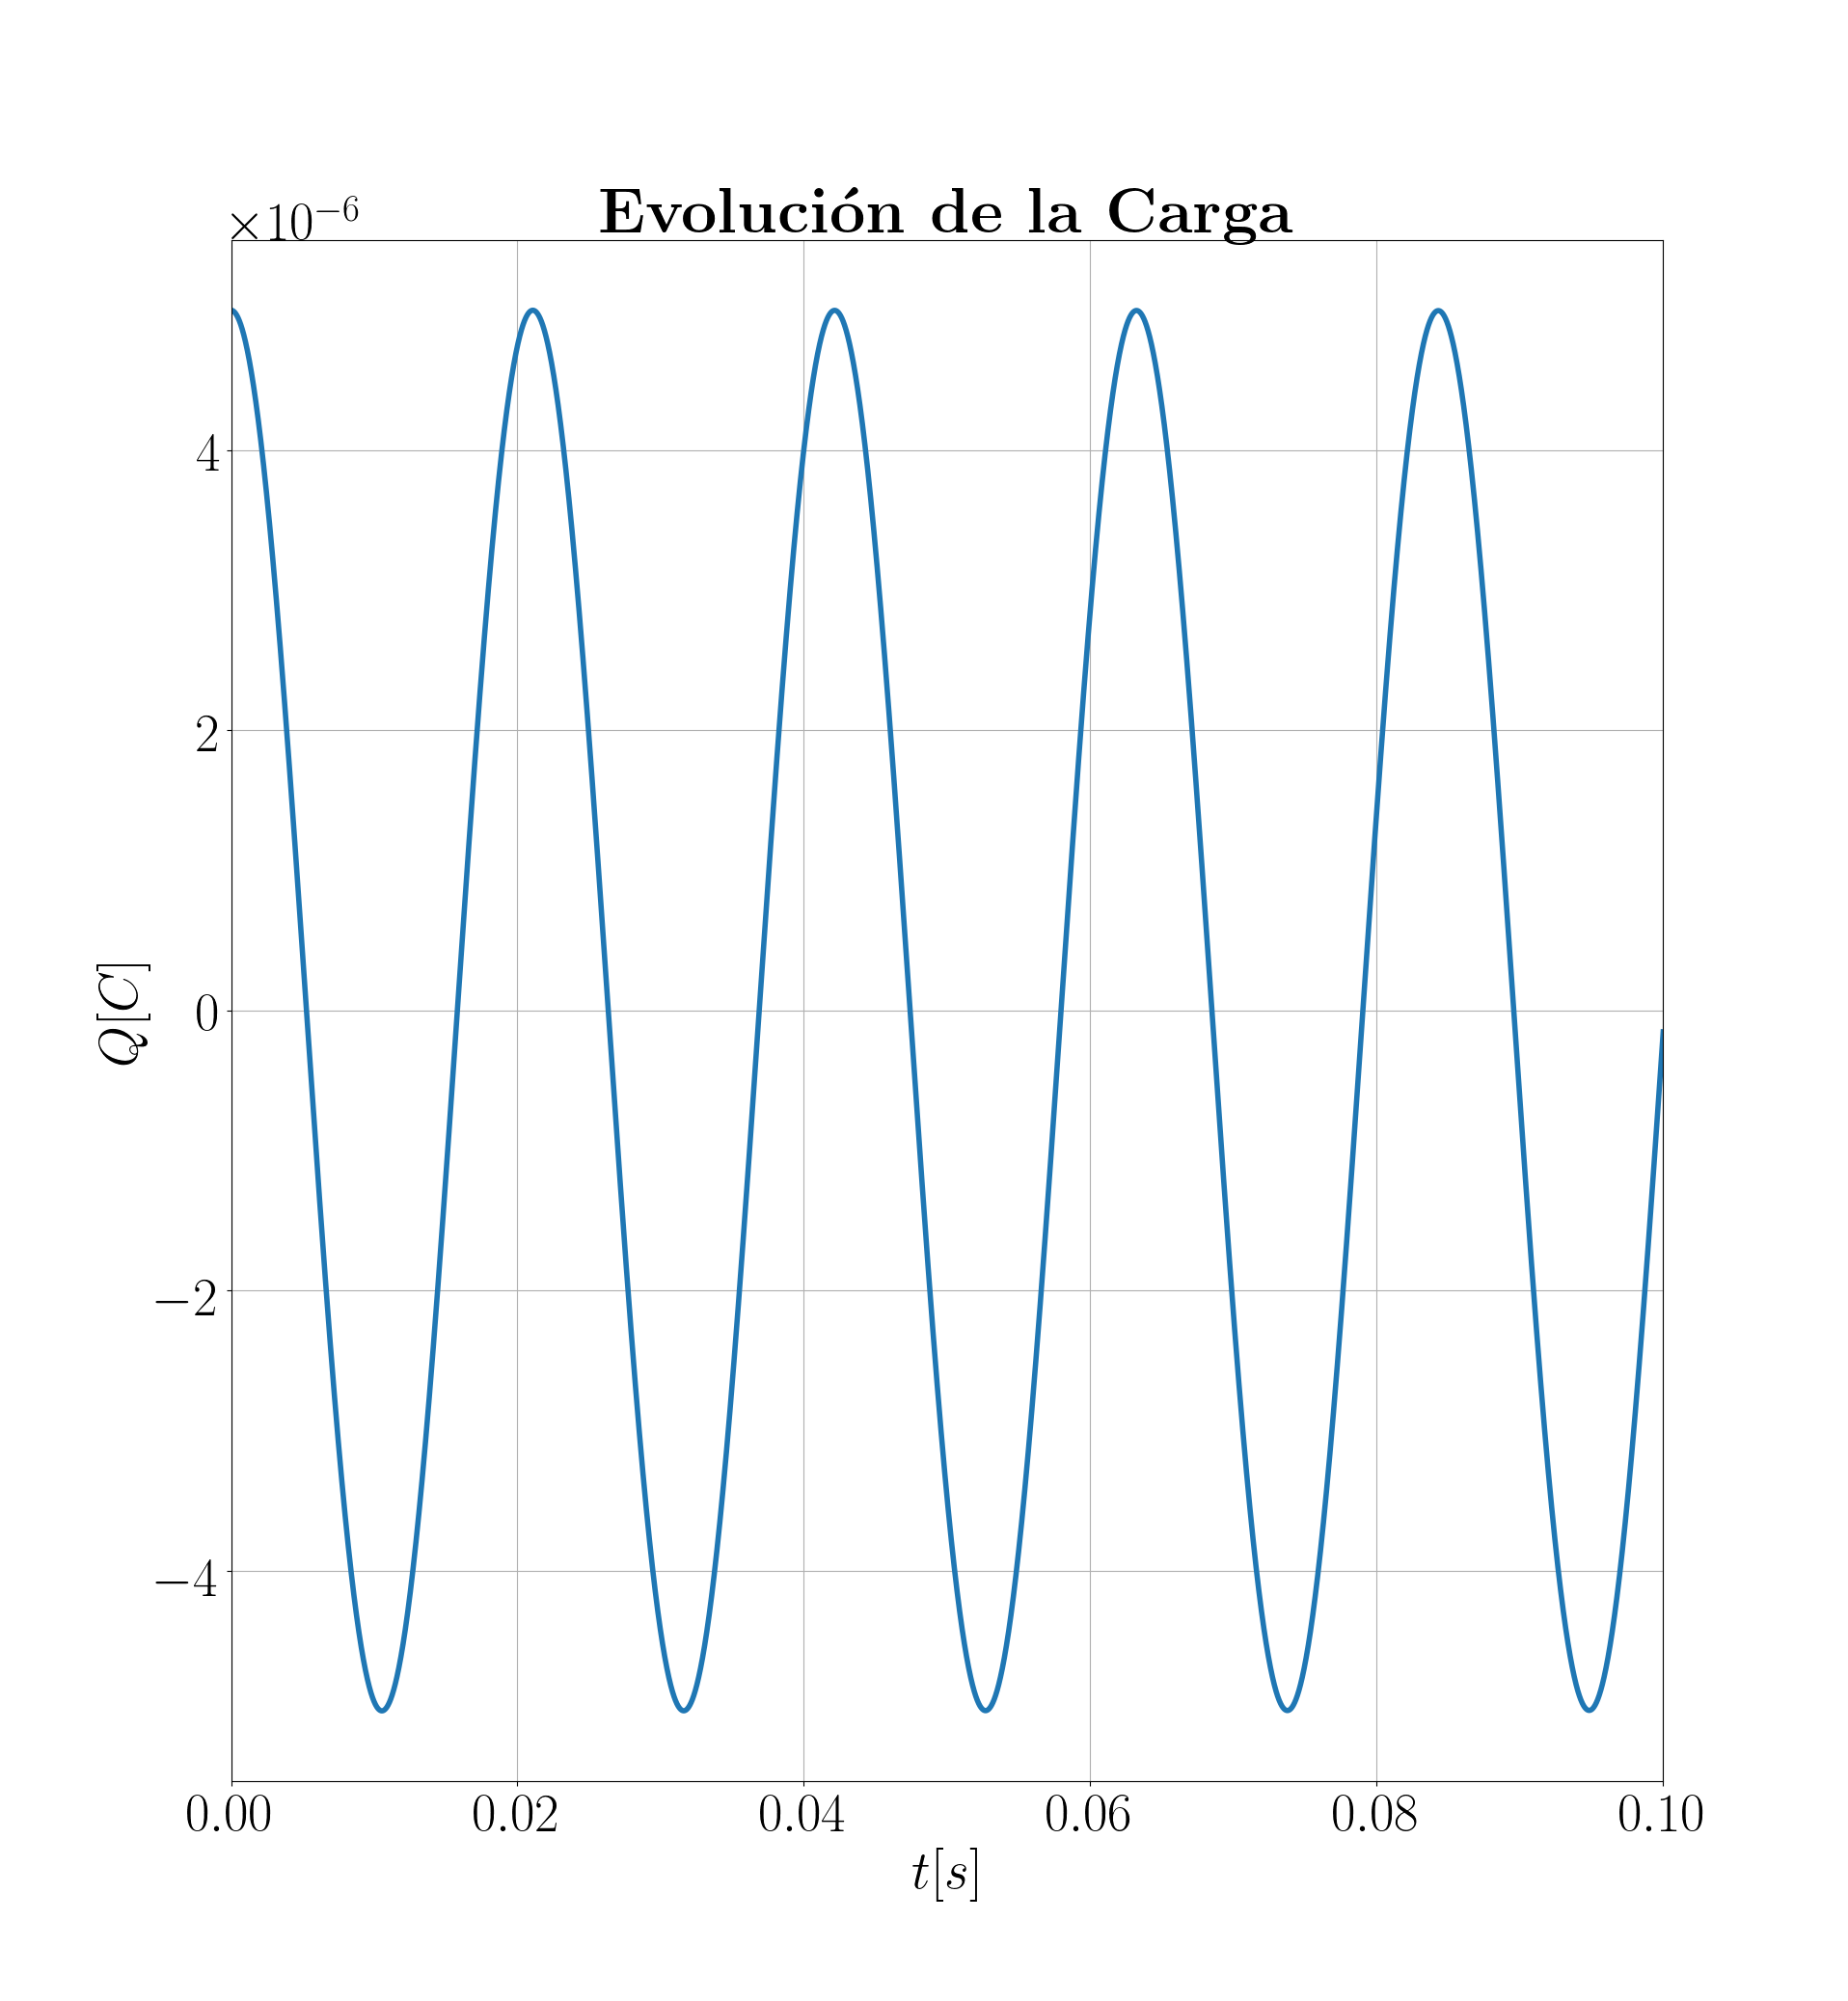
\includegraphics[width=\linewidth,trim={70 70 70 70},clip]{cargaamortiguado.png}
    \caption{Evolución temporal de la carga $Q~[C]$ en el caso del circuito $RLC$ amortiguado para $R=0~[\Omega]$ y con $tf=10.0~[s]$.}
    \label{fig:cargaamortiguado}
\end{figure}

\begin{figure}[!htb]
    \centering
    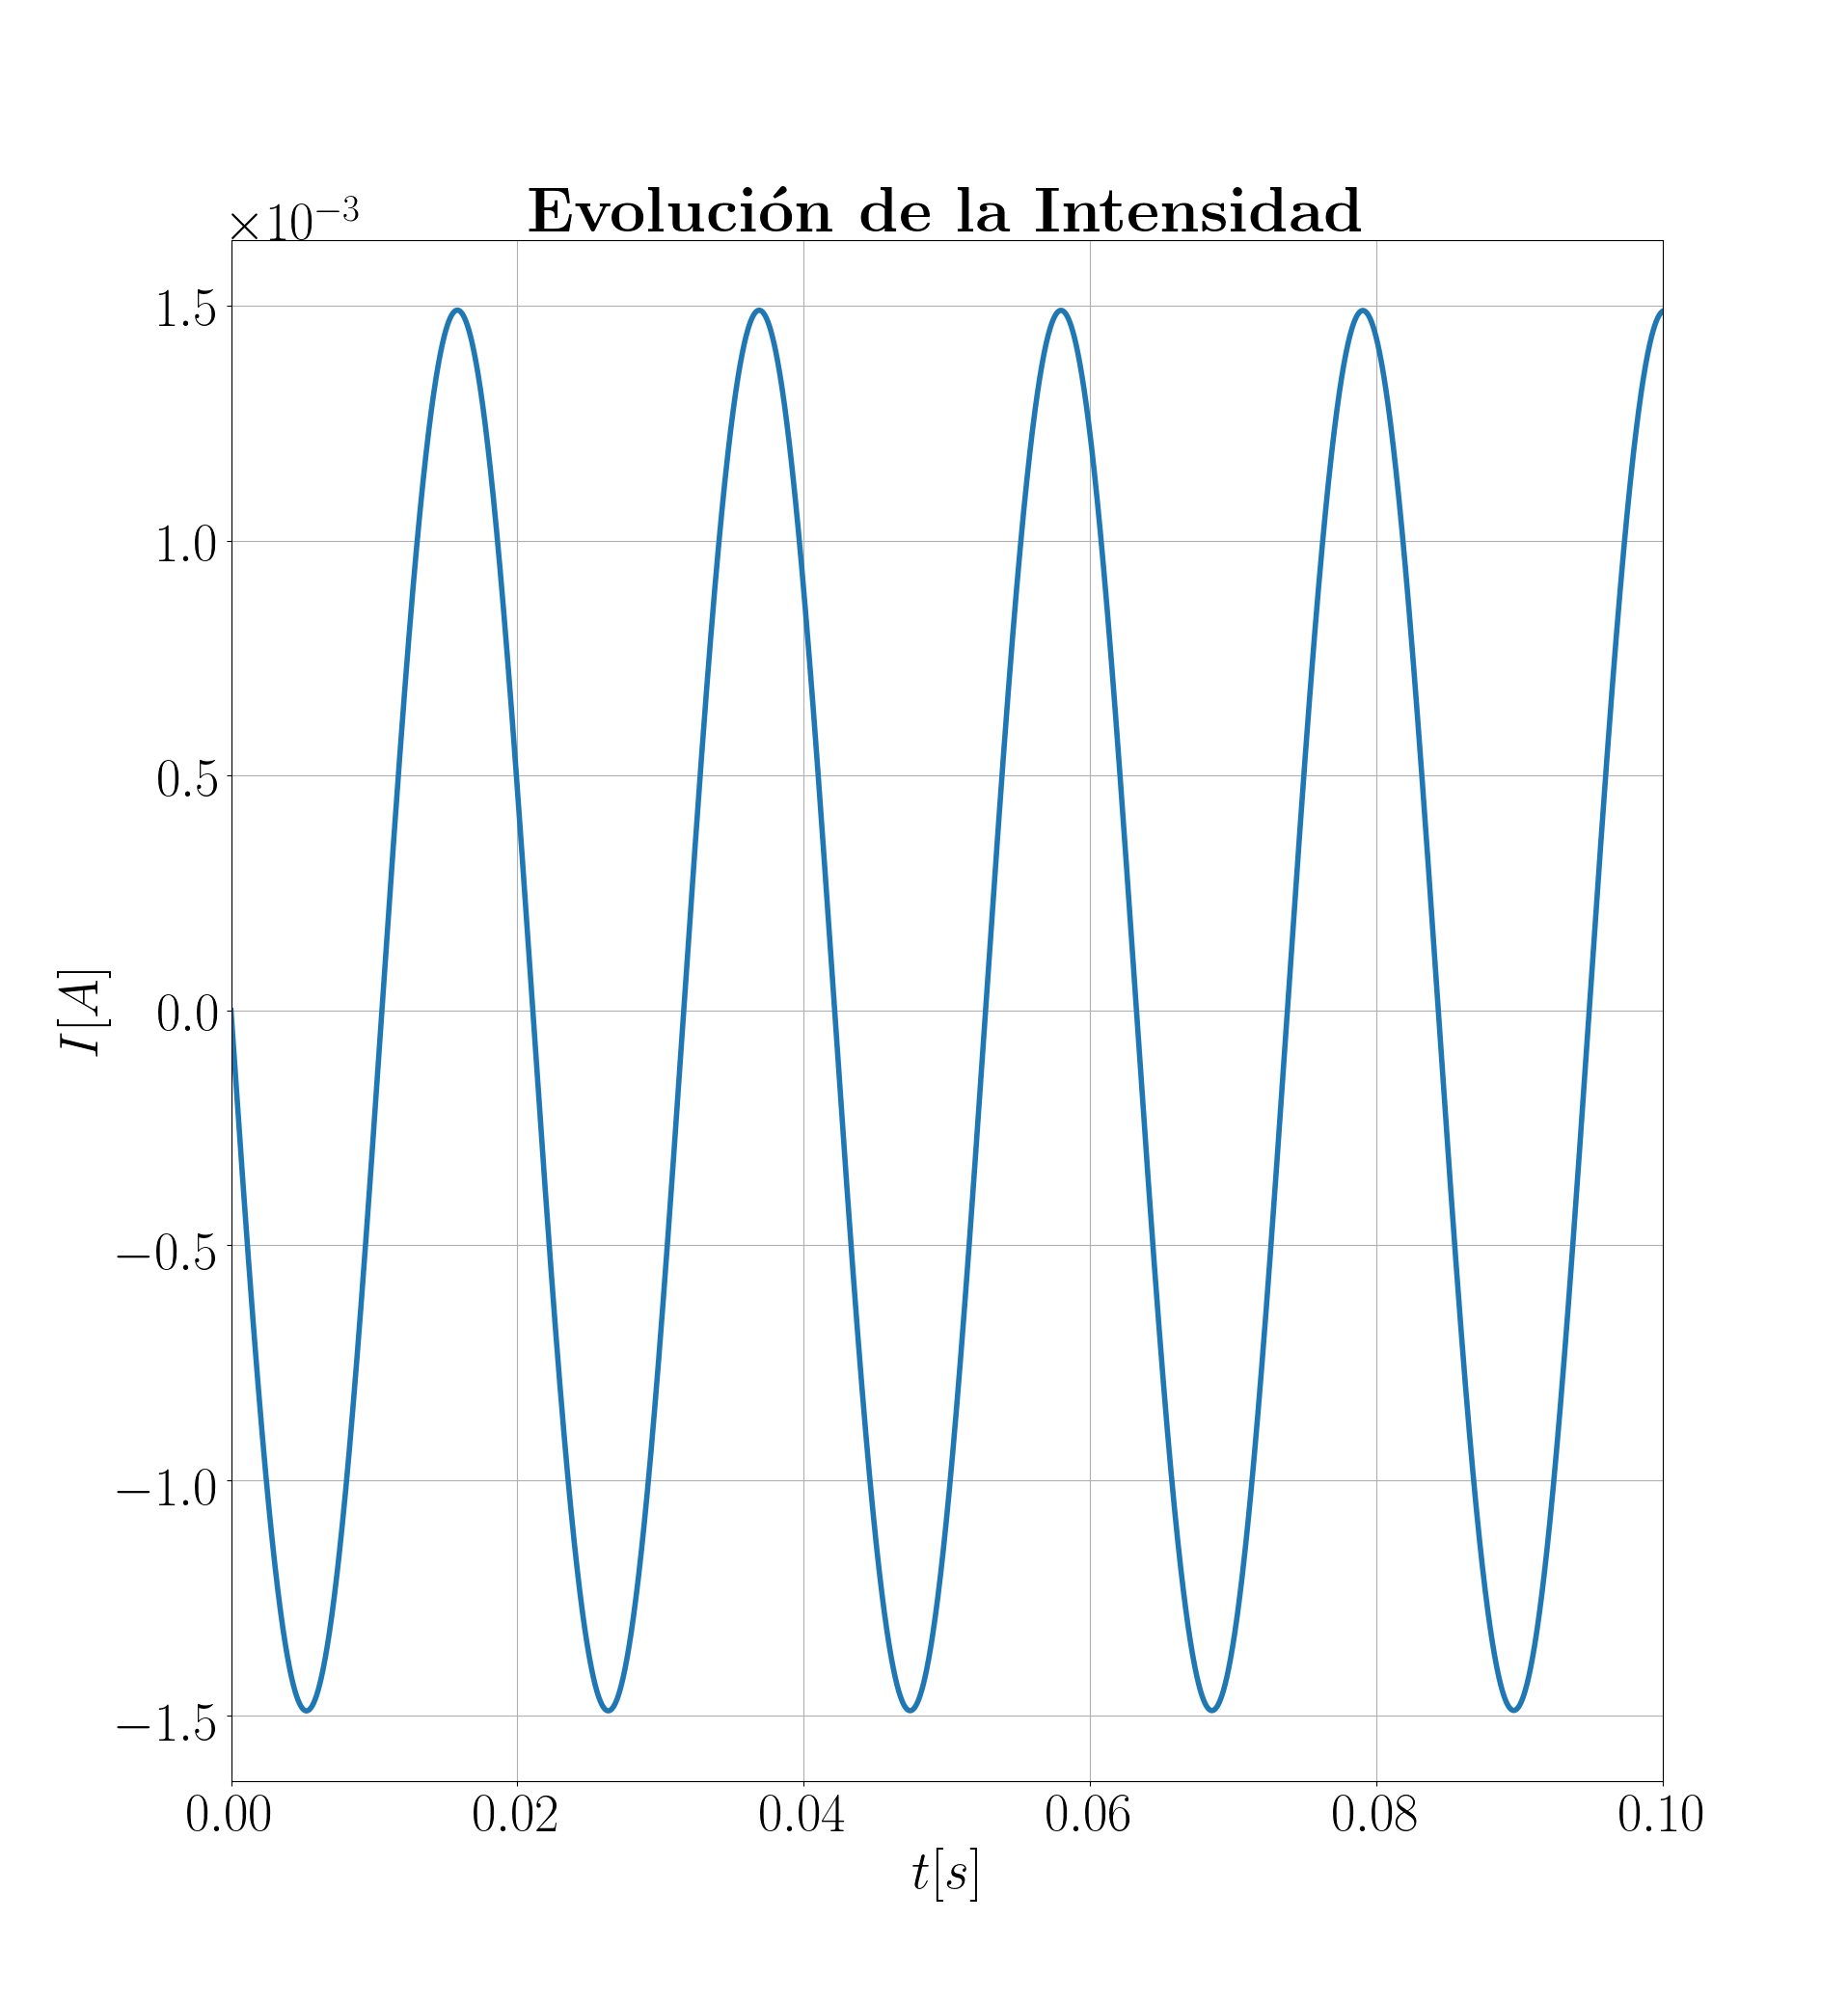
\includegraphics[width=\linewidth,trim={40 70 70 70},clip]{intensidadamortiguado.png}
    \caption{Evolución temporal de la intensidad $I~[A]$ en el caso del circuito $RLC$ amortiguado para $R=0~[\Omega]$ y con $tf=10.0~[s]$.}
    \label{fig:intensidadamortiguado}
\end{figure}

\newpage

Como podemos observar, en el caso amortiguado la evolución tanto de la carga como de la intensidad presentan el comportamiento de oscilación armónica amortiguada (una analogía típica es el péndulo sometido a rozamiento debido a la resistencia del aire). Así pues, la carga y la intensidad van a oscilar debido a la inversión de la carga en las placas del condensador.

La Figura \ref{fig:energiaamortiguado} muestra la evolución tanto de la energía magnética como electrostática y la suma de ambas. En ella podemos comprobar cómo cuando la carga $Q$ es nula toda la energía es magnética y está almacenada en el inductor (por ejemplo, en el instante $t=0.03$). De la misma forma, cuando la carga es máxima (instantes $t=0.02$ y $t=0.01$ aproximadamente), toda la energía es electrostática y está almacenada en el condensador.

\begin{figure}[!htb]
    \centering
    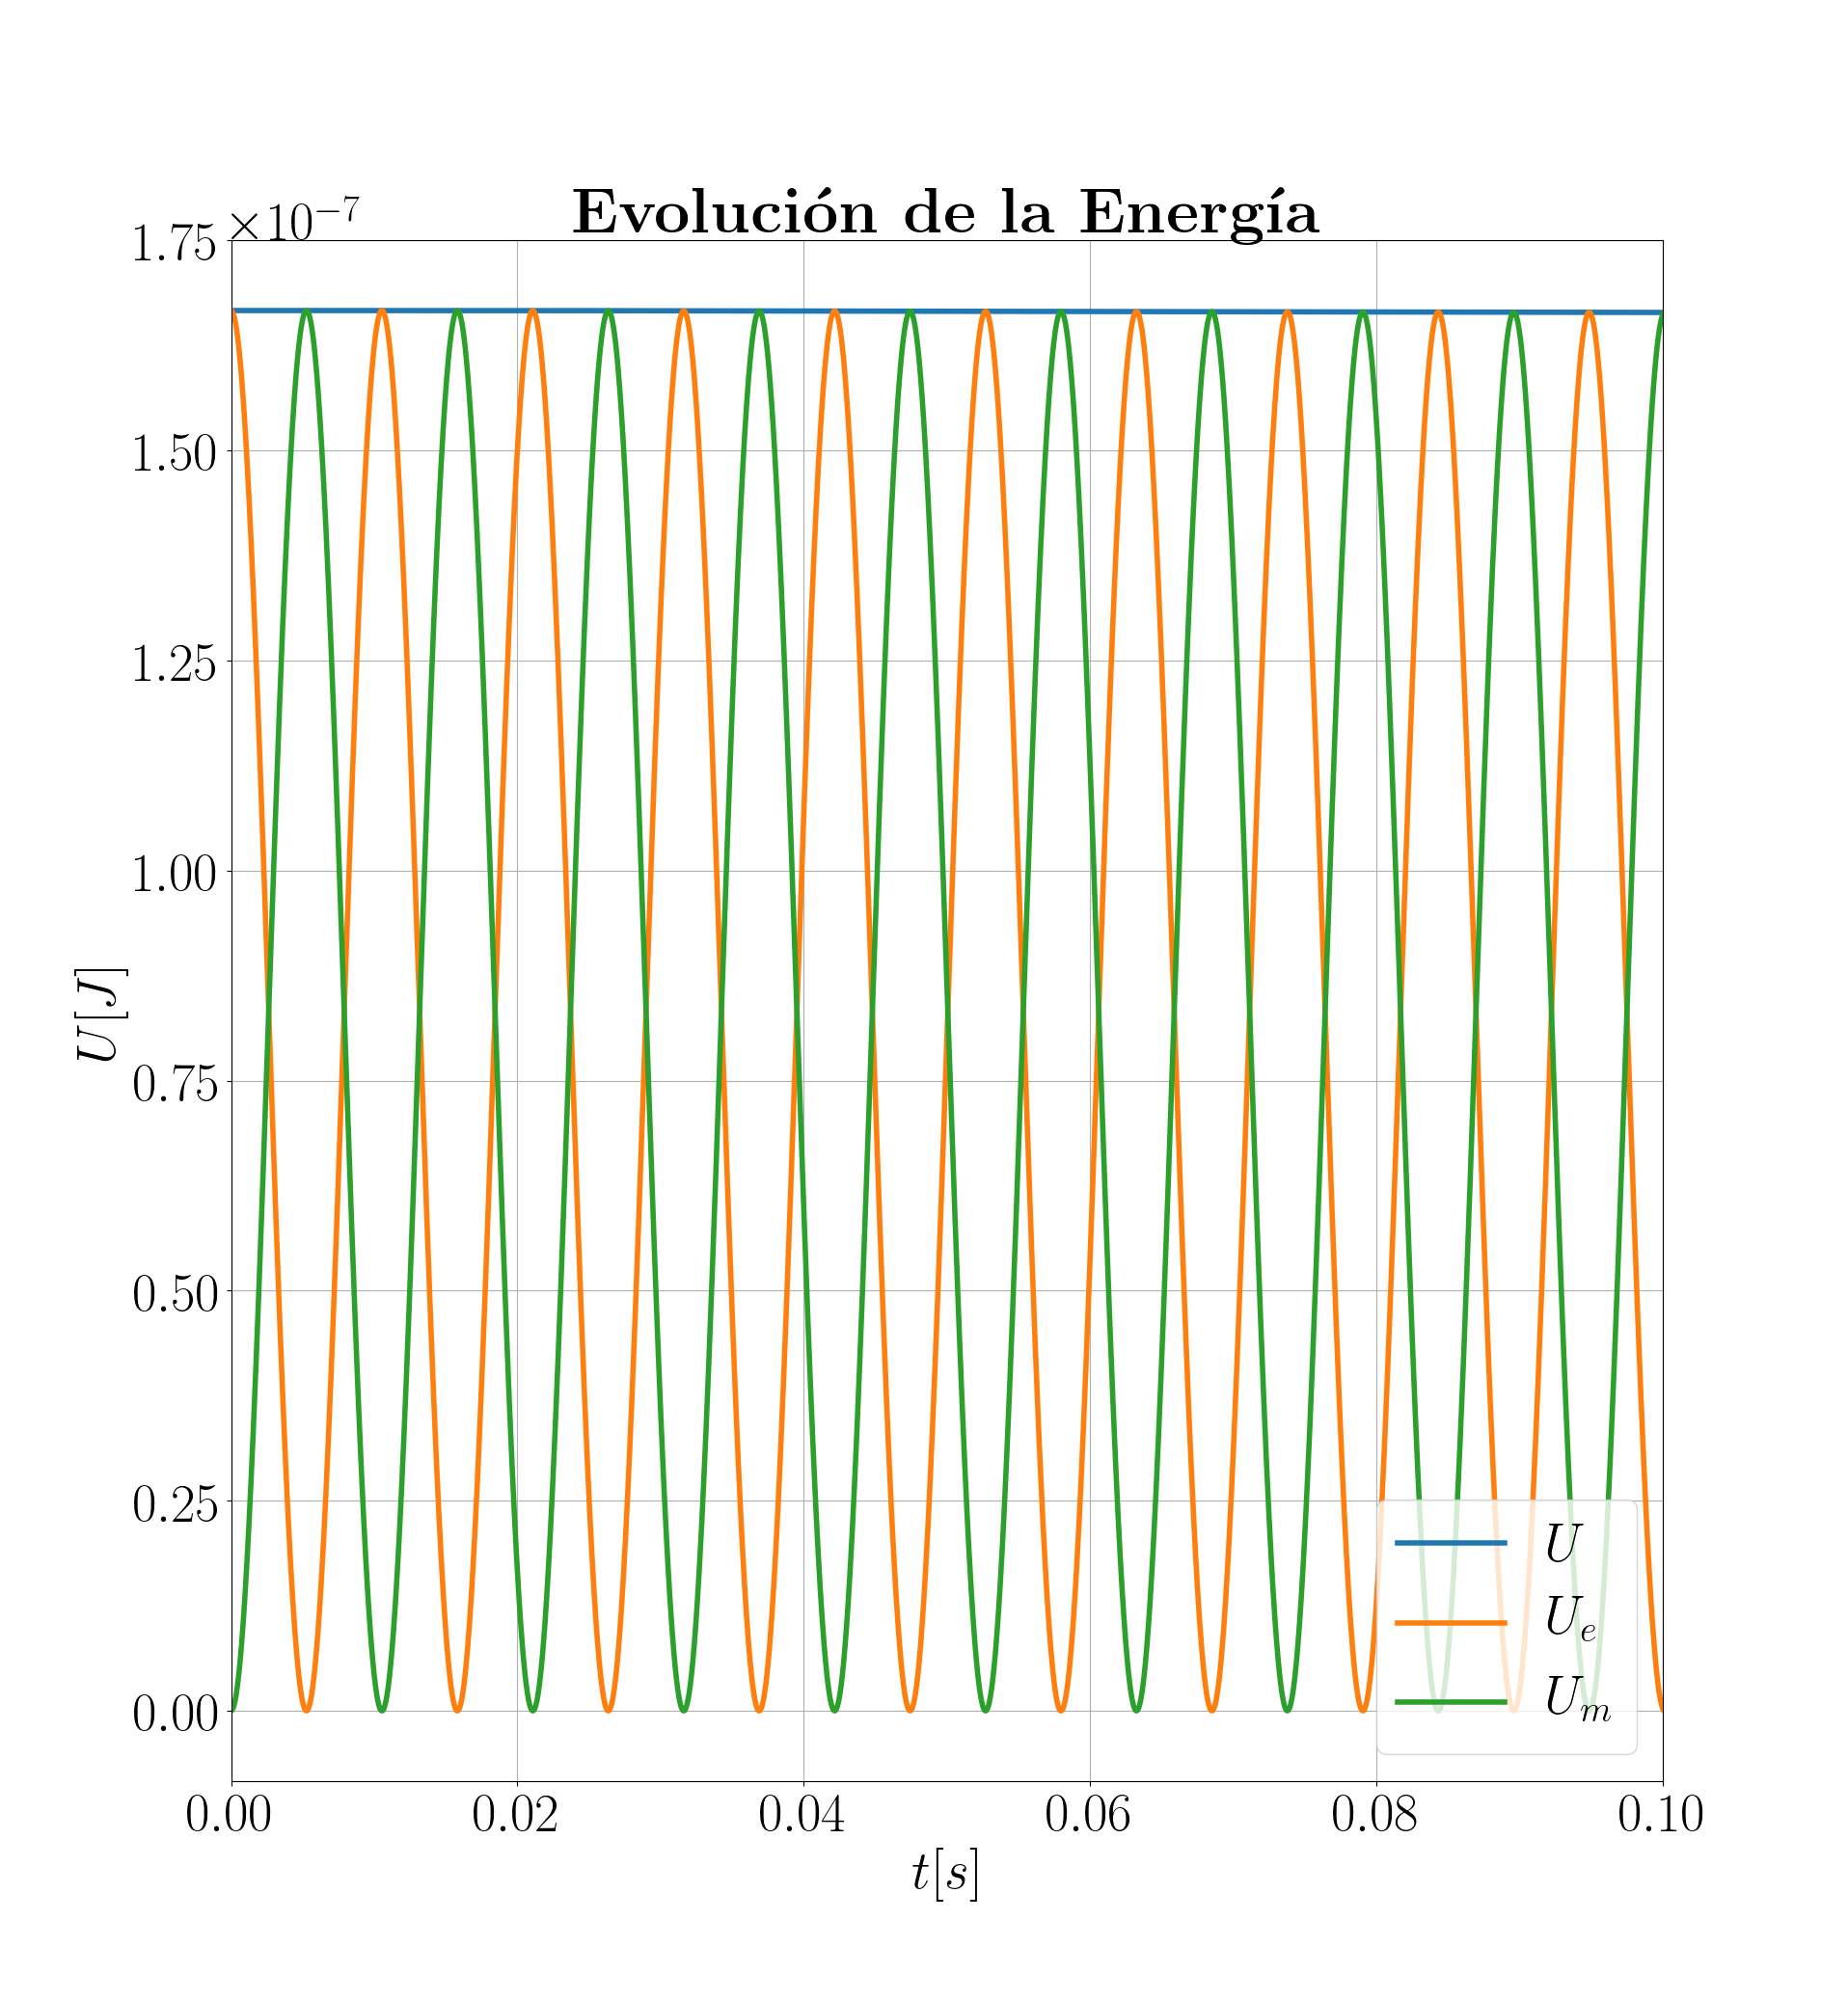
\includegraphics[width=\linewidth,trim={40 70 70 70},clip]{energiaamortiguado.png}
    \caption{Evolución de las energías magnética $U_m$, electrostática $U_e$ y total $U$ en el caso amortiguado para $R=0~[\Omega]$.}
    \label{fig:energiaamortiguado}
\end{figure}

De forma teórica, la frecuencia de oscilación es:

\begin{equation}
f = \frac{1}{2\pi\sqrt{LC}} = \frac{1}{2\pi\sqrt{(0.15 \cdot 75.0 \cdot 10^{-6})}} = 47.45~[Hz]
\end{equation}

Atendiendo a la gráfica de la evolución de la carga $Q~[C]$ mostrada en la Figura \ref{fig:cargaamortiguado}, podemos determinar que el período de oscilación (tiempo transcurrido entre dos máximos) es aproximadamente de $T = 0.021~[s]$ ya que el primer máximo lo encontramos en $t=0.000~[s]$ y el siguiente en $t\simeq 0.021~[s]$. Dado que la frecuencia es la inversa del período $f = 1/T$, la frecuencia obtenida a partir de la gráfica es $f = 1 / 0.021 = 47.62$, la cual, apreciando los errores de precisión al seleccionar los valores de la gráfica, coincide con la frecuencia teórica calculada.

\clearpage

\subsection{Oscilador Subamortiguado}
\label{subsec:osciladorsubamortiguado}

Analizado el caso del oscilador amortiguado, procederemos a estudiar la situación subamortiguada. Para ello, mantendremos los mismos valores de $C$, $L$ y $Q_0$ mientras que cambiaremos el valor para la resistencia $R$. Para darse la situación subamortiguada necesitamos la siguiente condición

\begin{equation}
R^2 < \frac{4L}{C}~[\Omega]~.
\end{equation}

Así pues, elegimos un valor para $R$

\begin{equation}
R = 0.1 \cdot \sqrt{\frac{4L}{C}} = 0.1\cdot\sqrt{\frac{4\cdot 0.15}{75.00\cdot10^{-6}}} = 8.94~[\Omega]~.
\end{equation}

Una vez determinado un valor necesario de $R~[\Omega]$ para producir la subamortiguación, ejecutamos de nuevo el programa \mintinline{c}{RLC.py} y obtenemos las gráficas de evolución de la carga $Q~[C]$ (Figura \ref{fig:cargasubamortiguado}), de la intensidad (Figura \ref{fig:intensidadsubamortiguado}) y de energía (Figura \ref{fig:energiasubamortiguado}).

\begin{figure}[!htb]
    \centering
    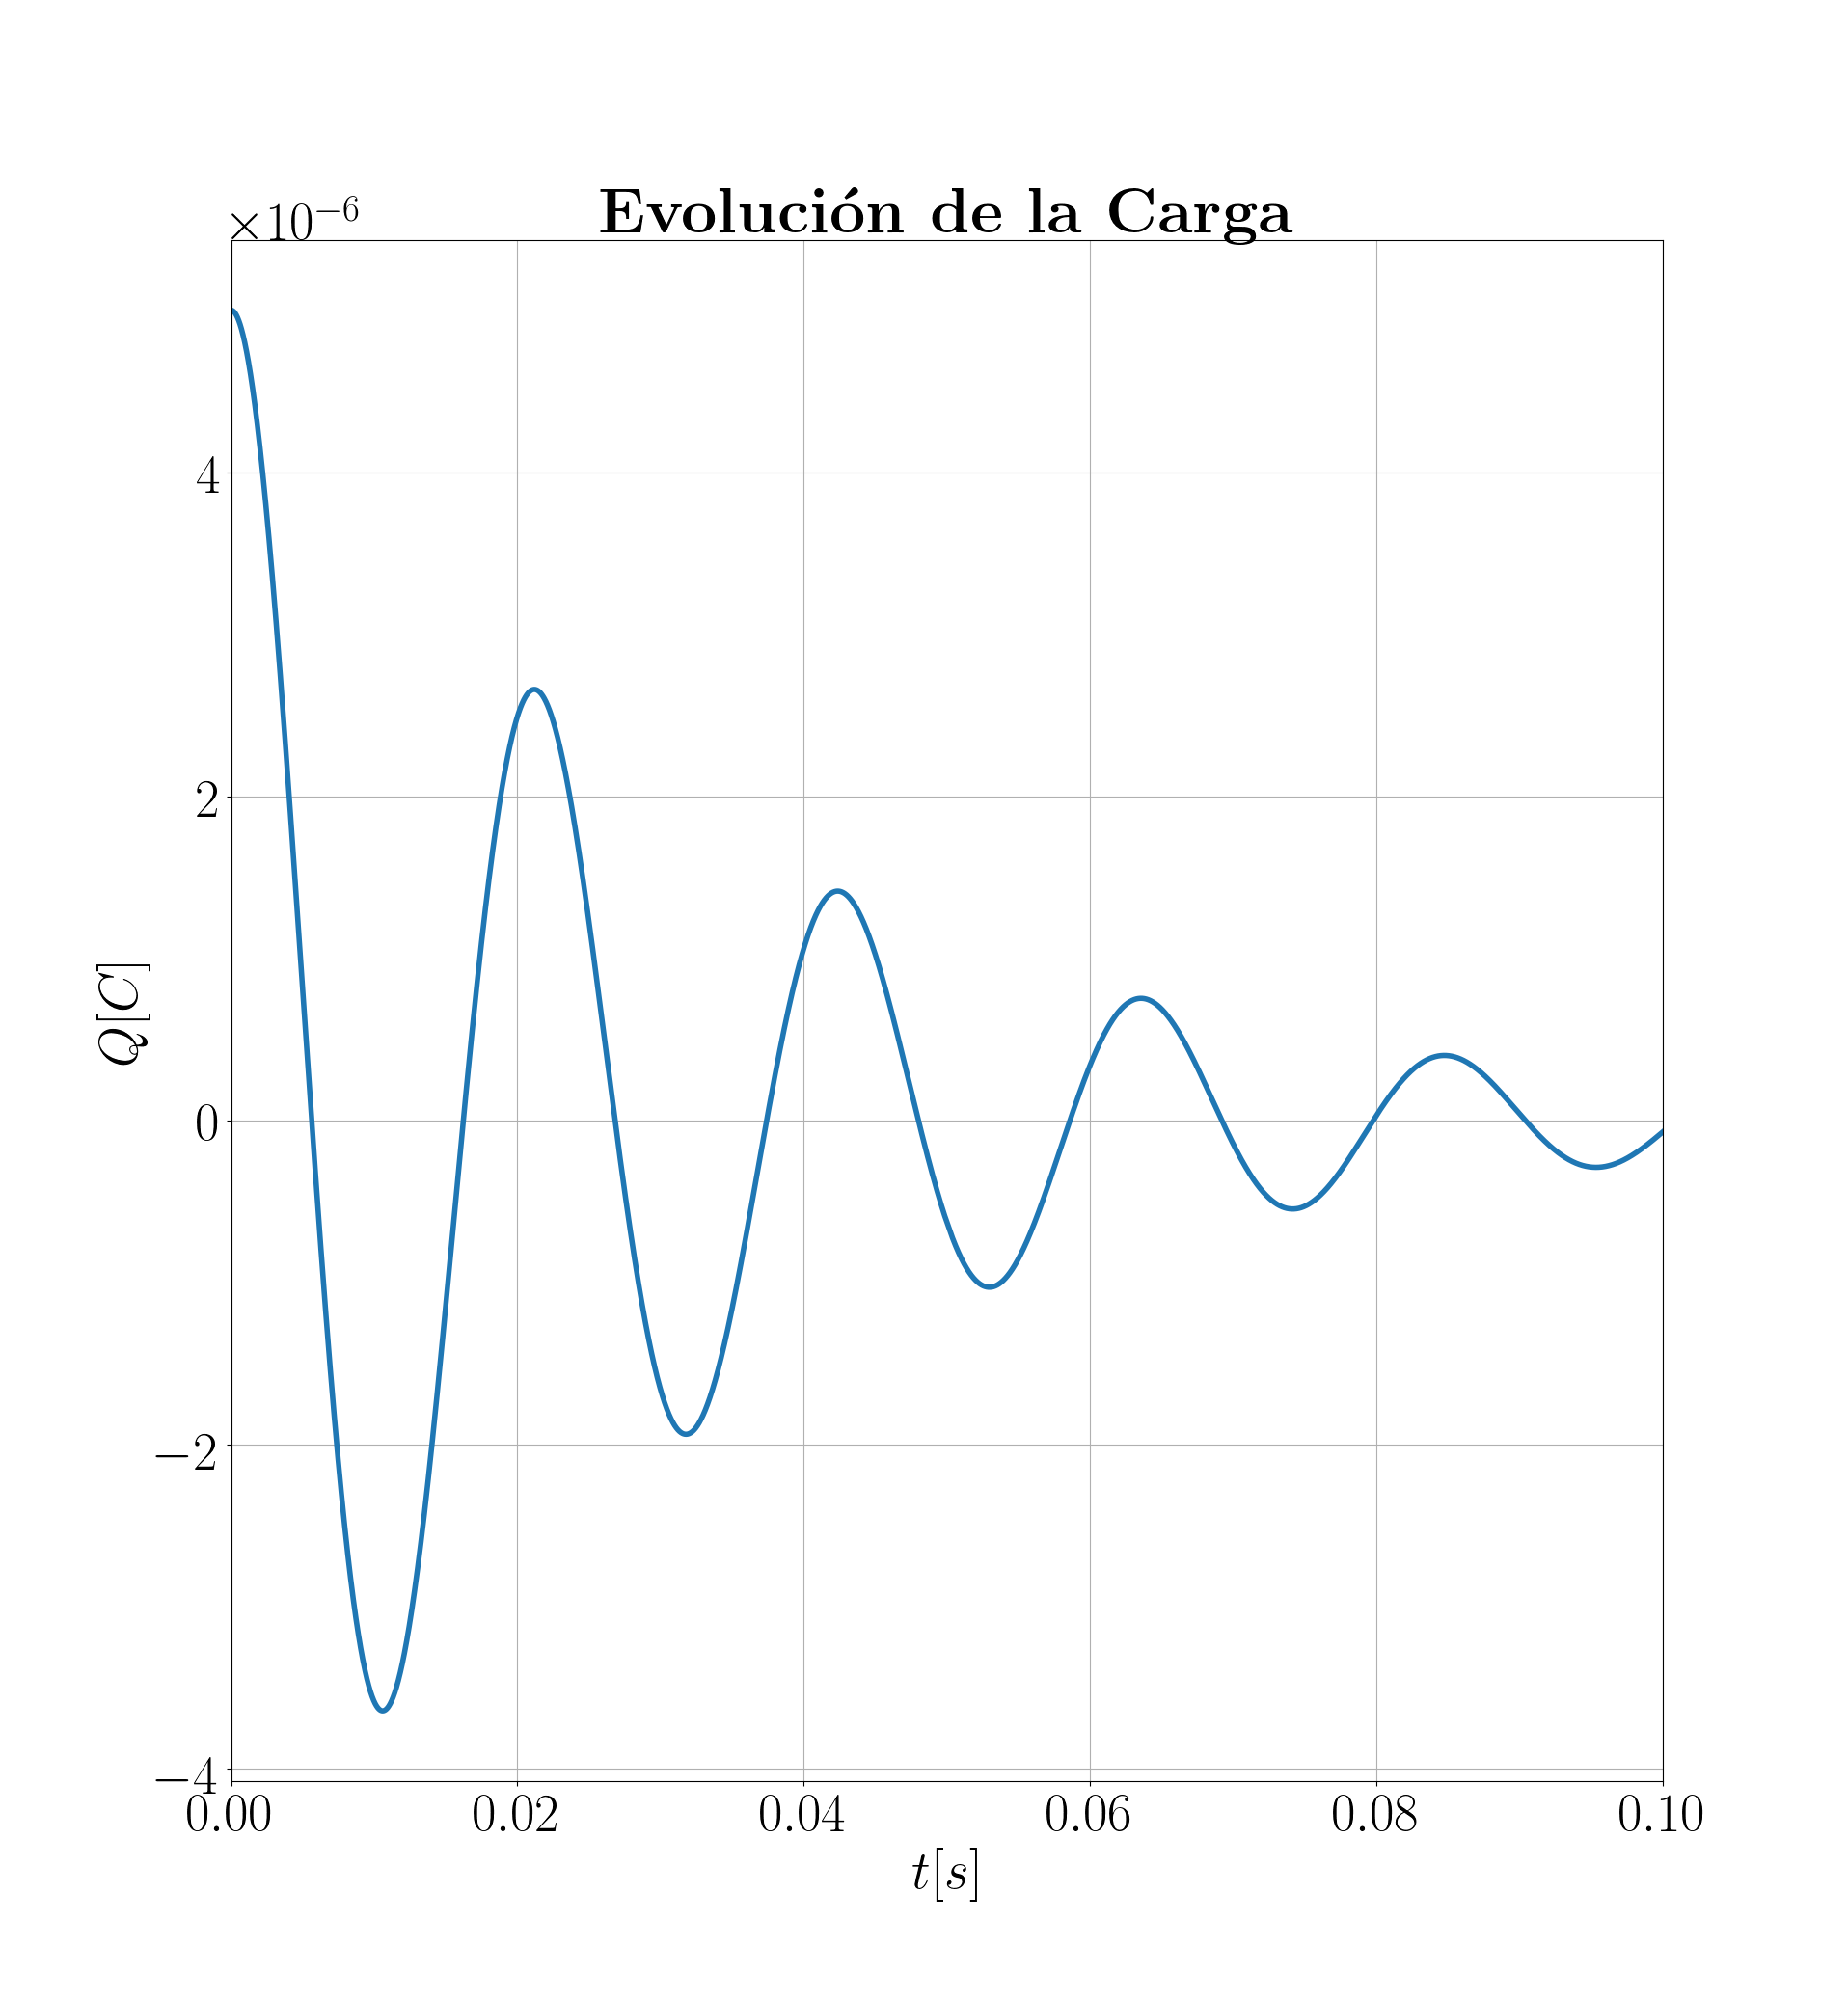
\includegraphics[width=\linewidth,trim={70 70 70 105},clip]{cargasubamortiguado.png}
    \caption{Evolución de la carga $Q~[C]$ en el caso subamortiguado para $R=0.1 \cdot\sqrt{\frac{4L}{C}}~[\Omega]$.}
    \label{fig:cargasubamortiguado}
\end{figure}

En este caso podemos observar cómo, aunque se sigue produciendo oscilación con el mismo comportamiento que en el caso anterior, la amplitud de la misma disminuye con el tiempo lo cual provoca una disminución progresiva del valor absoluto de la carga, de la intensidad y por lo tanto una disminución de la energía del sistema a medida que transcurre el tiempo. Dicha energía se pierde progresivamente a causa principalmente de la resistencia.

\begin{figure}[!htb]
    \centering
    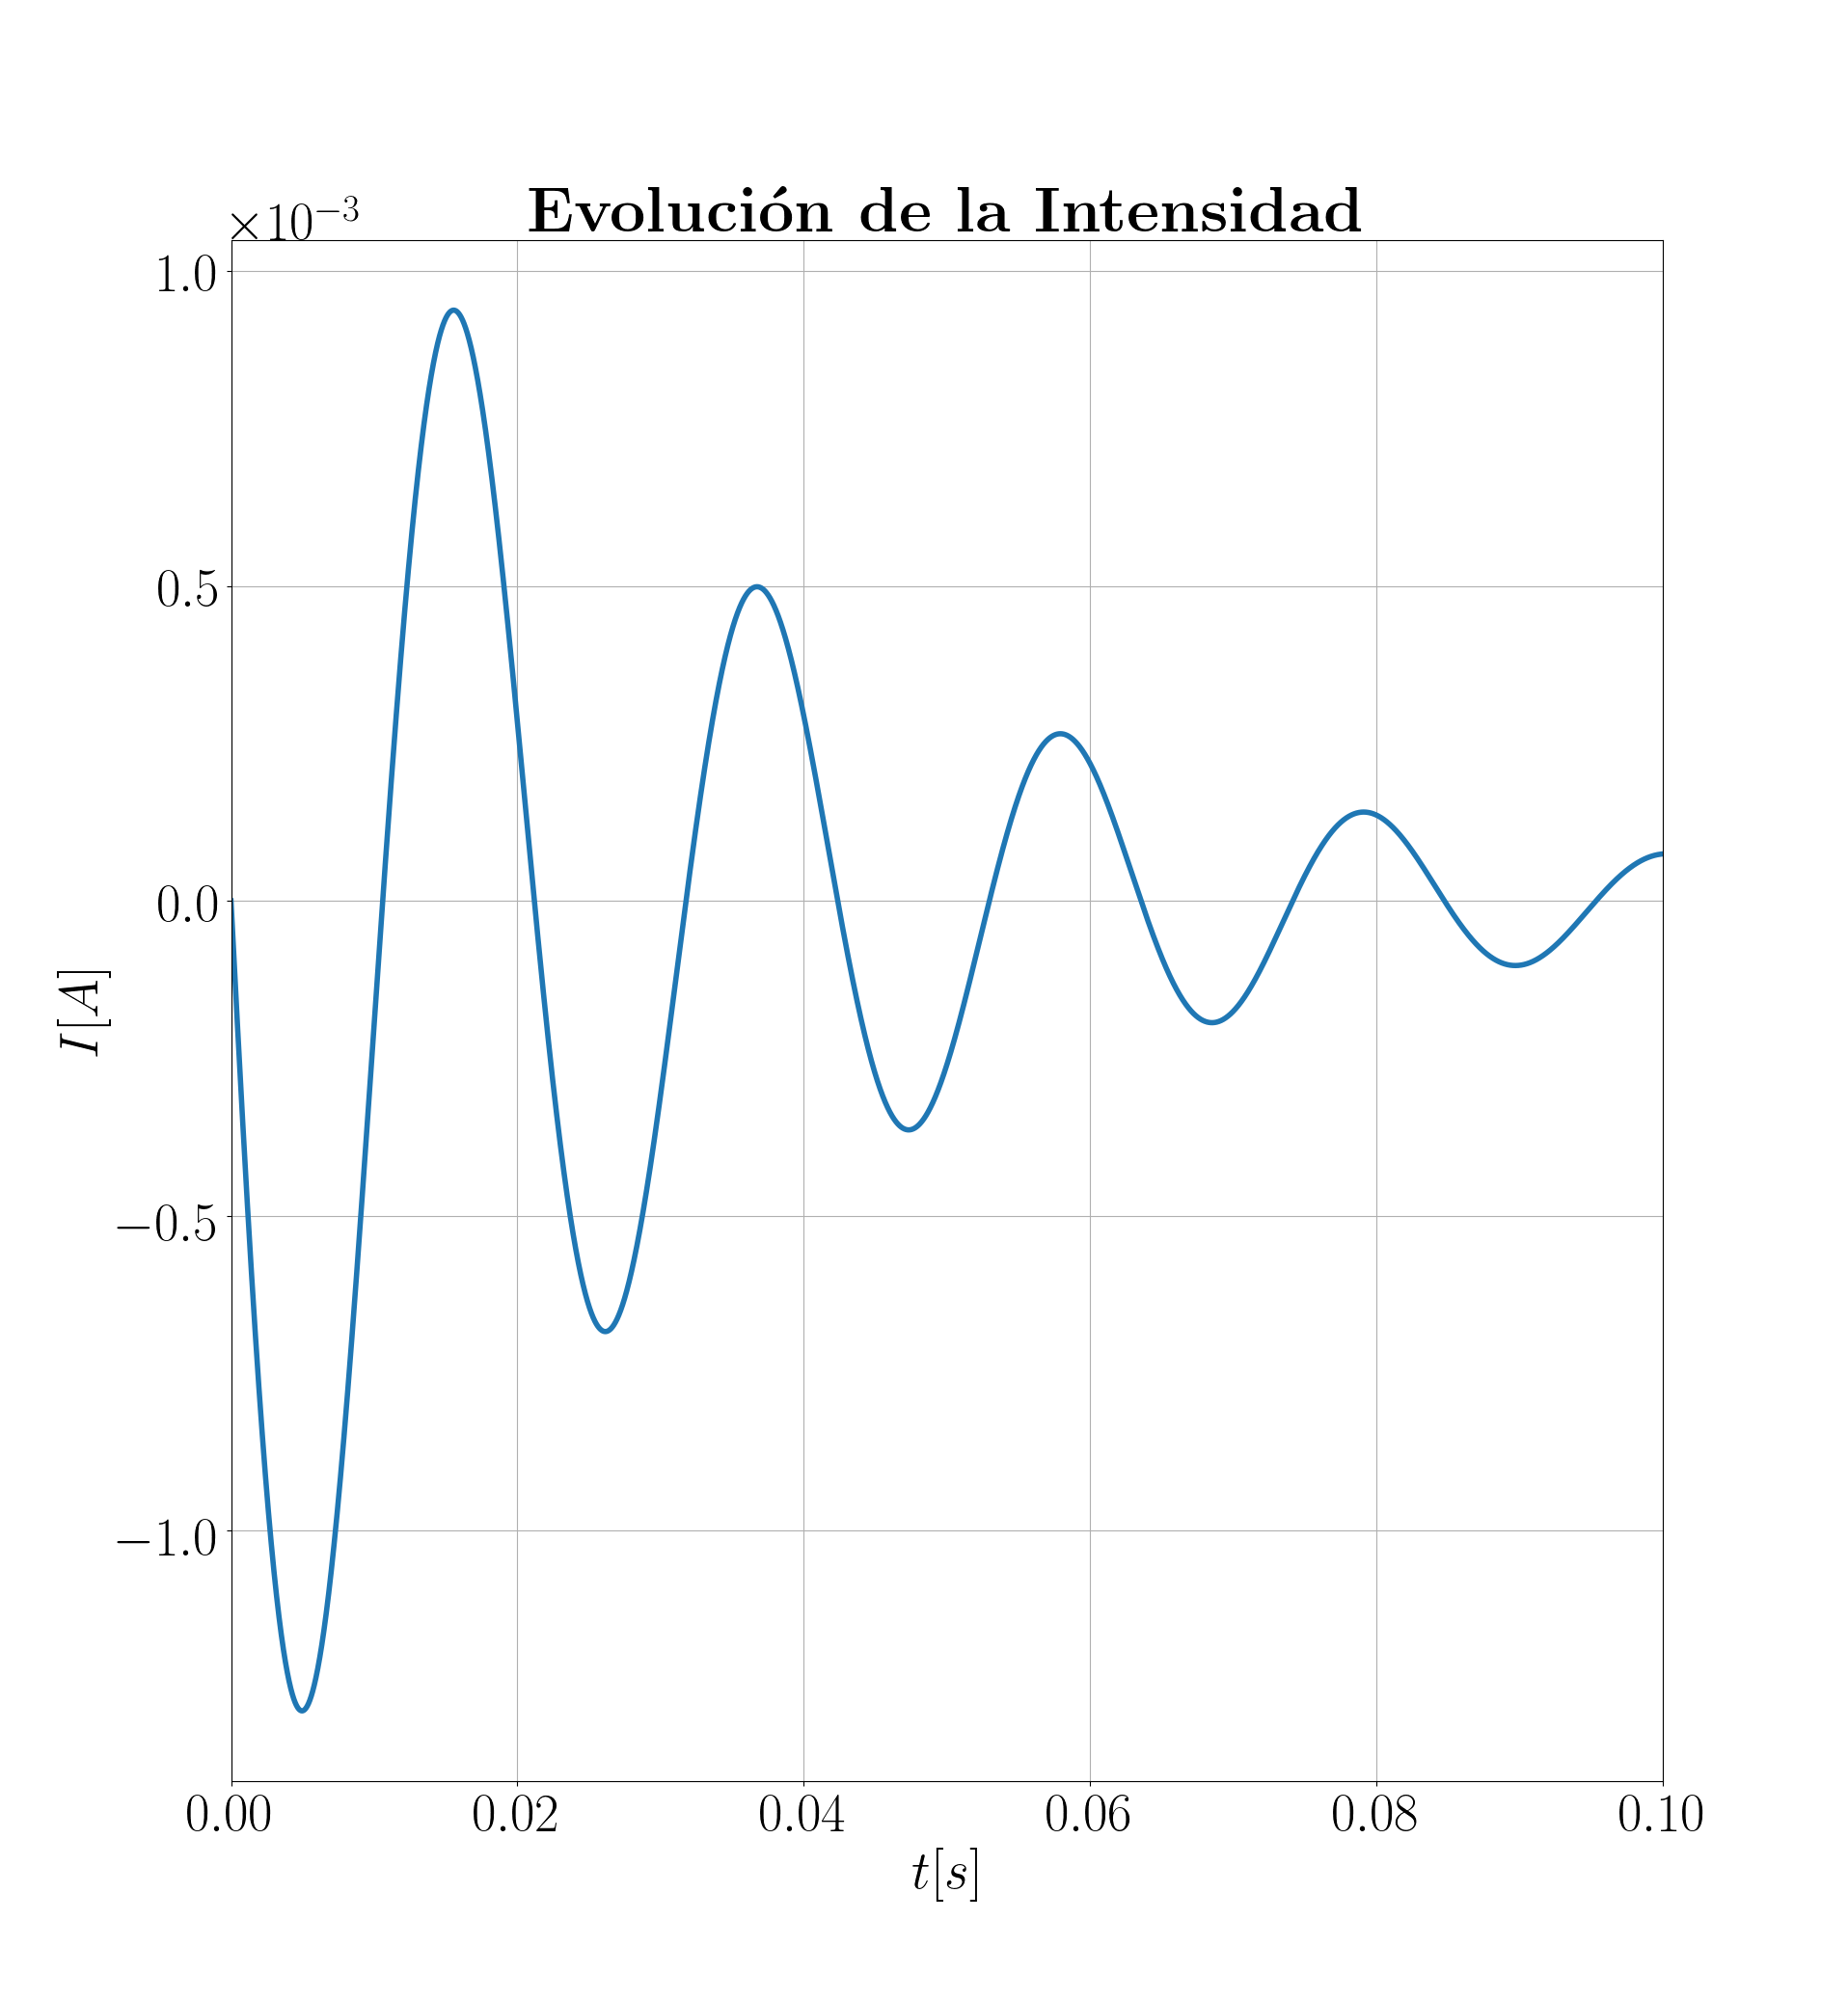
\includegraphics[width=\linewidth,trim={40 70 70 105},clip]{intensidadsubamortiguado.png}
    \caption{Evolución de la intensidad $I~[A]$ en el caso subamortiguado para $R=0.1 \cdot\sqrt{\frac{4L}{C}}~[\Omega]$.}
    \label{fig:intensidadsubamortiguado}
\end{figure}

En este caso, la frecuencia de oscilación no cambia respecto al caso anterior ($f = 47.45~[Hz]$) dado que la misma únicamente depende de $L$ y de $C$. Como se puede comprobar en la Figura \ref{fig:cargaamortiguado}, de la misma forma que en la Figura \ref{fig:cargaamortiguado}, el período de oscilación entre los primeros dos máximos ($t = 0.000~[s]$ y $t \simeq 0.021~[s]$) es $T = 0.021~[s]$. Por lo tanto, la frecuencia es $f = 1/0.021 = 47.62~[Hz]$.

\begin{figure}[!htb]
    \centering
    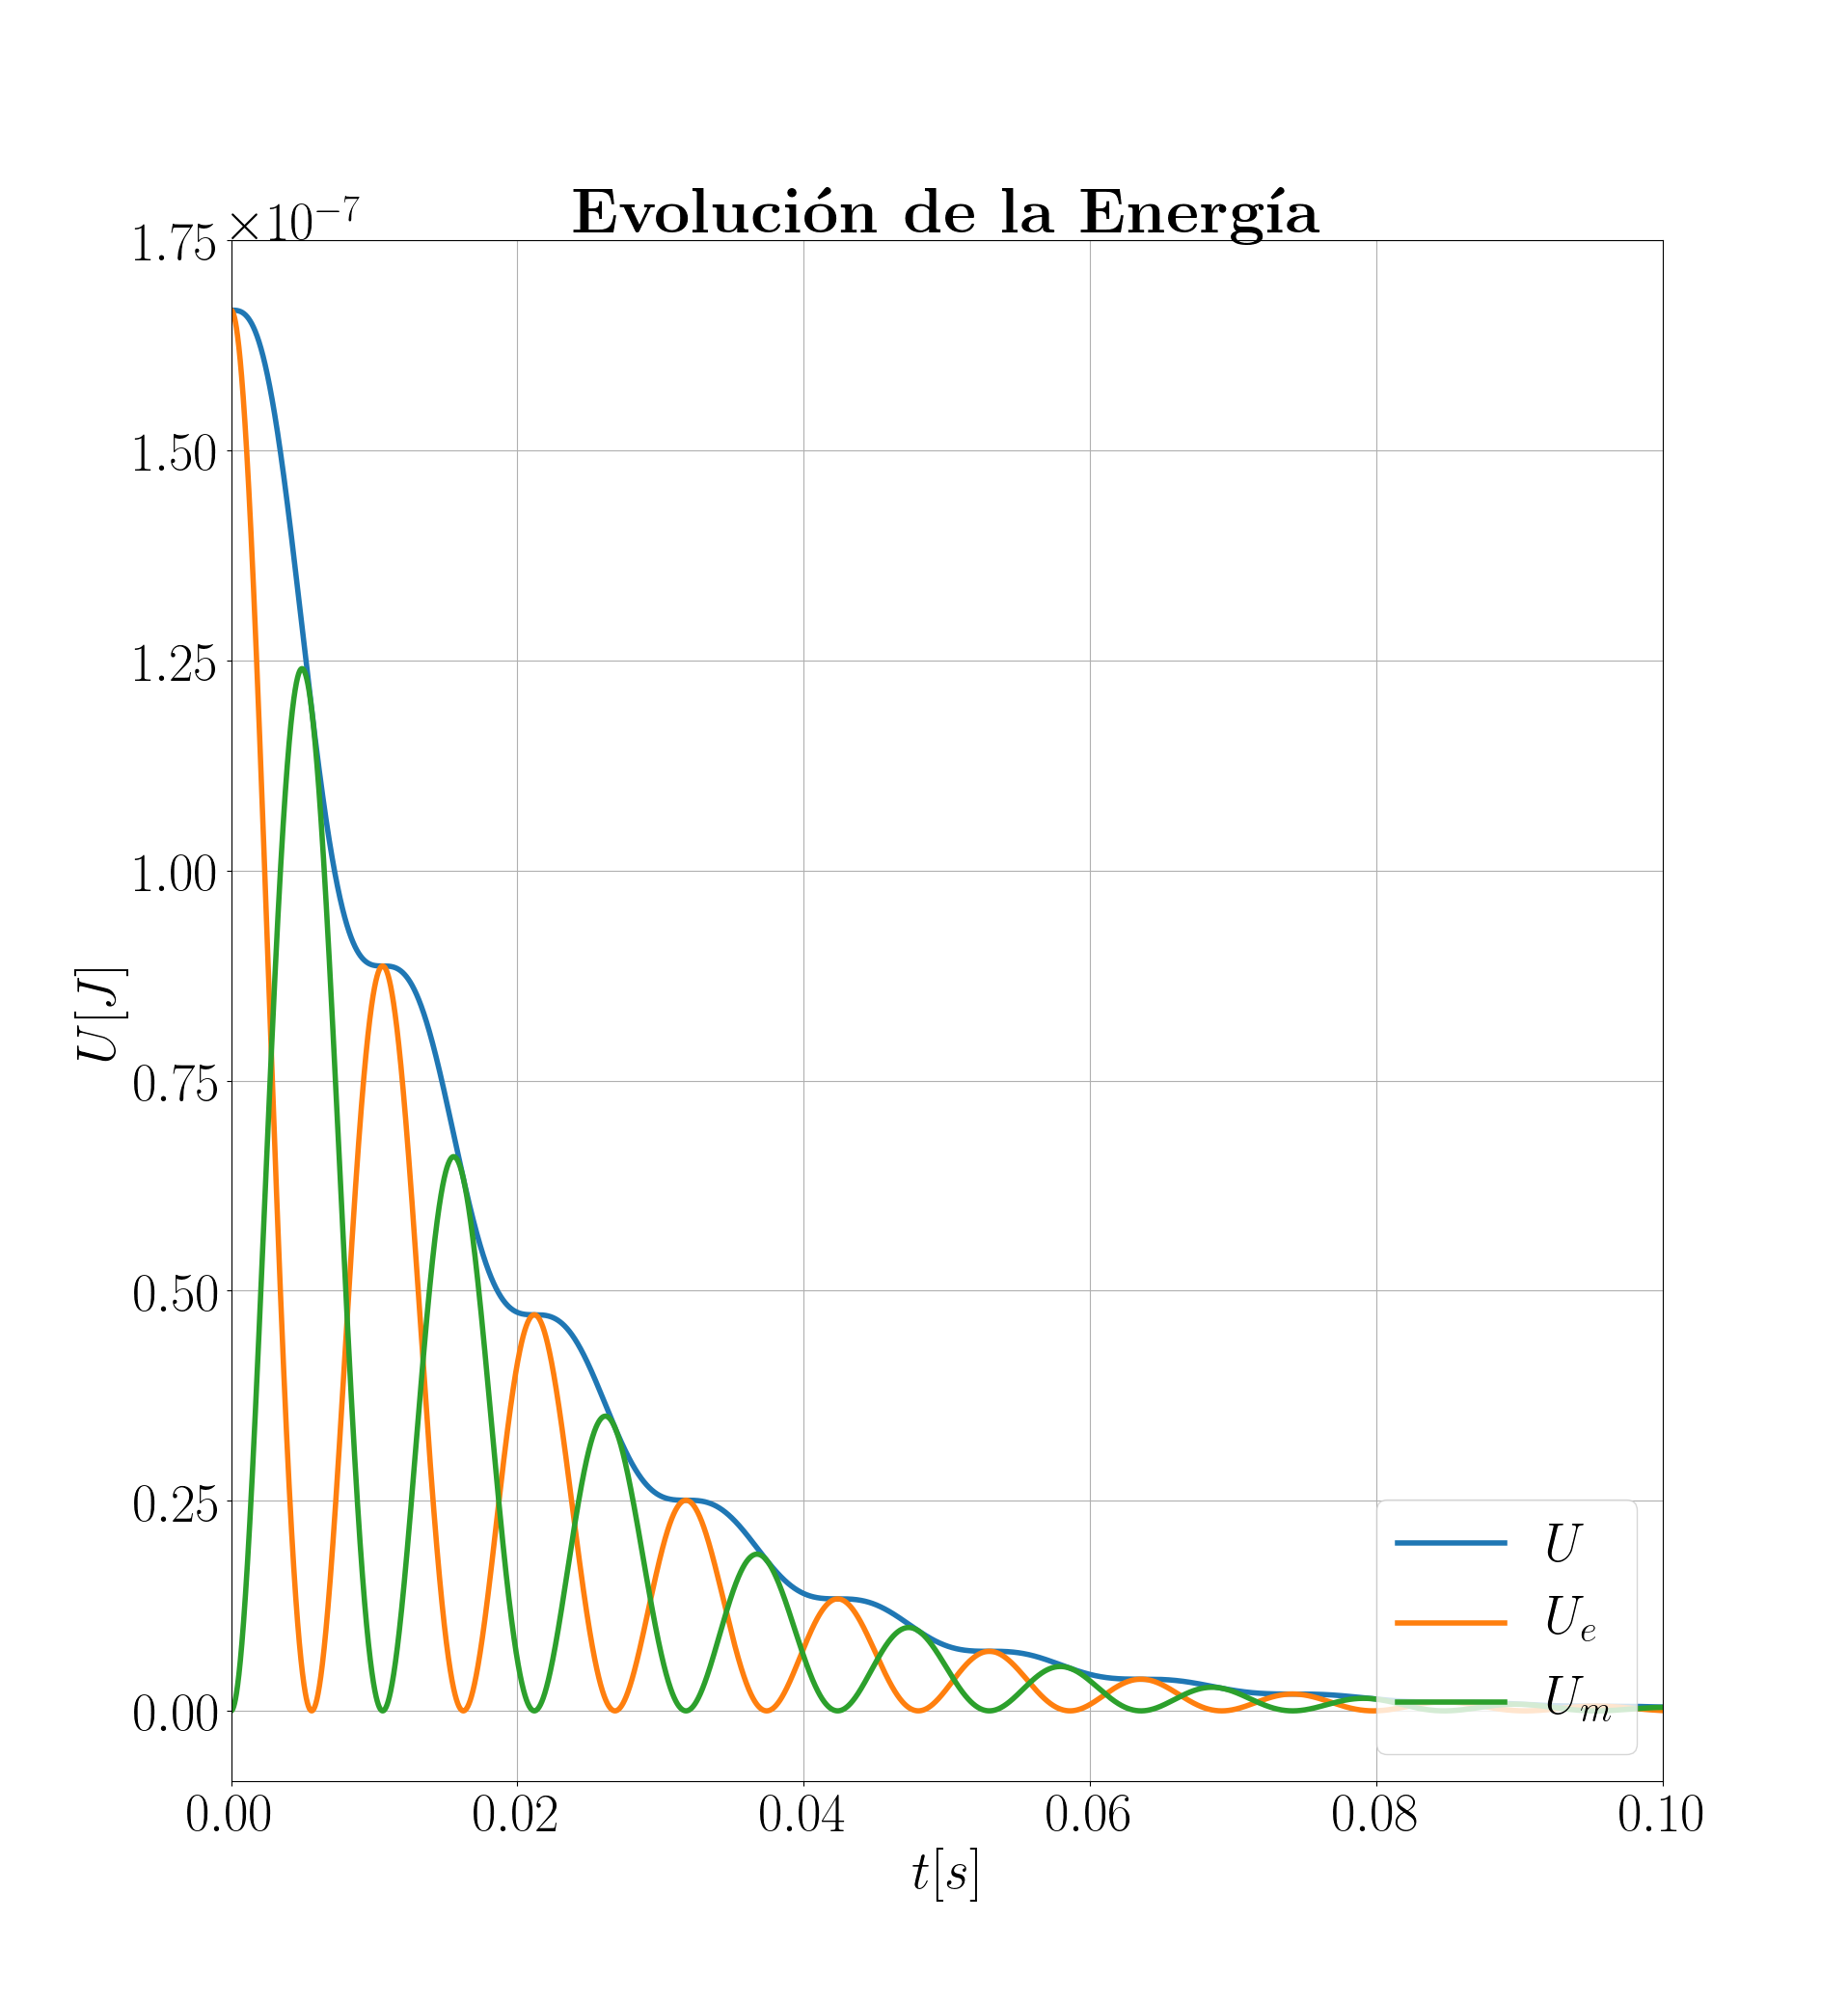
\includegraphics[width=\linewidth,trim={40 70 70 105},clip]{energiasubamortiguado.png}
    \caption{Evolución de las energías magnética $U_m$, electrostática $U_e$ y total $U$ en el caso subamortiguado para $R=0.1 \cdot\sqrt{\frac{4L}{C}}~[\Omega]$.}
    \label{fig:energiasubamortiguado}
\end{figure}

\clearpage

\subsection{Oscilador Sobreamortiguado}
\label{subsec:osciladorsobreamortiguado}

Por último, simularemos el caso sobreamortiguado. De nuevo, mantenemos los mismos valores para el condensador $C$, la bobina $L$ y para la carga inicial $Q_0$ y cambiaremos el valor de la resistencia $R$. Para conseguir una situación de sobreamortiguación debe cumplirse que

\begin{equation}
R^2 > \frac{4L}{C}~[\Omega]~,
\end{equation}

por lo que daremos un valor arbitrario a $R$ de 

\begin{equation}
R = 10 \cdot \sqrt{\frac{4L}{C}} = 0.1\cdot\sqrt{\frac{4\cdot 0.15}{75.00\cdot10^{-6}}} = 894.43~[\Omega]~.
\end{equation}

Determinado un valor necesario de $R~[\Omega]$ para producir la sobreamortiguación, ejecutamos de nuevo el programa \mintinline{c}{RLC.py} y obtenemos las gráficas de evolución de la carga $Q~[C]$ (Figura \ref{fig:cargasobreamortiguado}), de la intensidad (Figura \ref{fig:intensidadsobreamortiguado}) y de energía (Figura \ref{fig:energiasobreamortiguado}).

\begin{figure}[!htb]
    \centering
    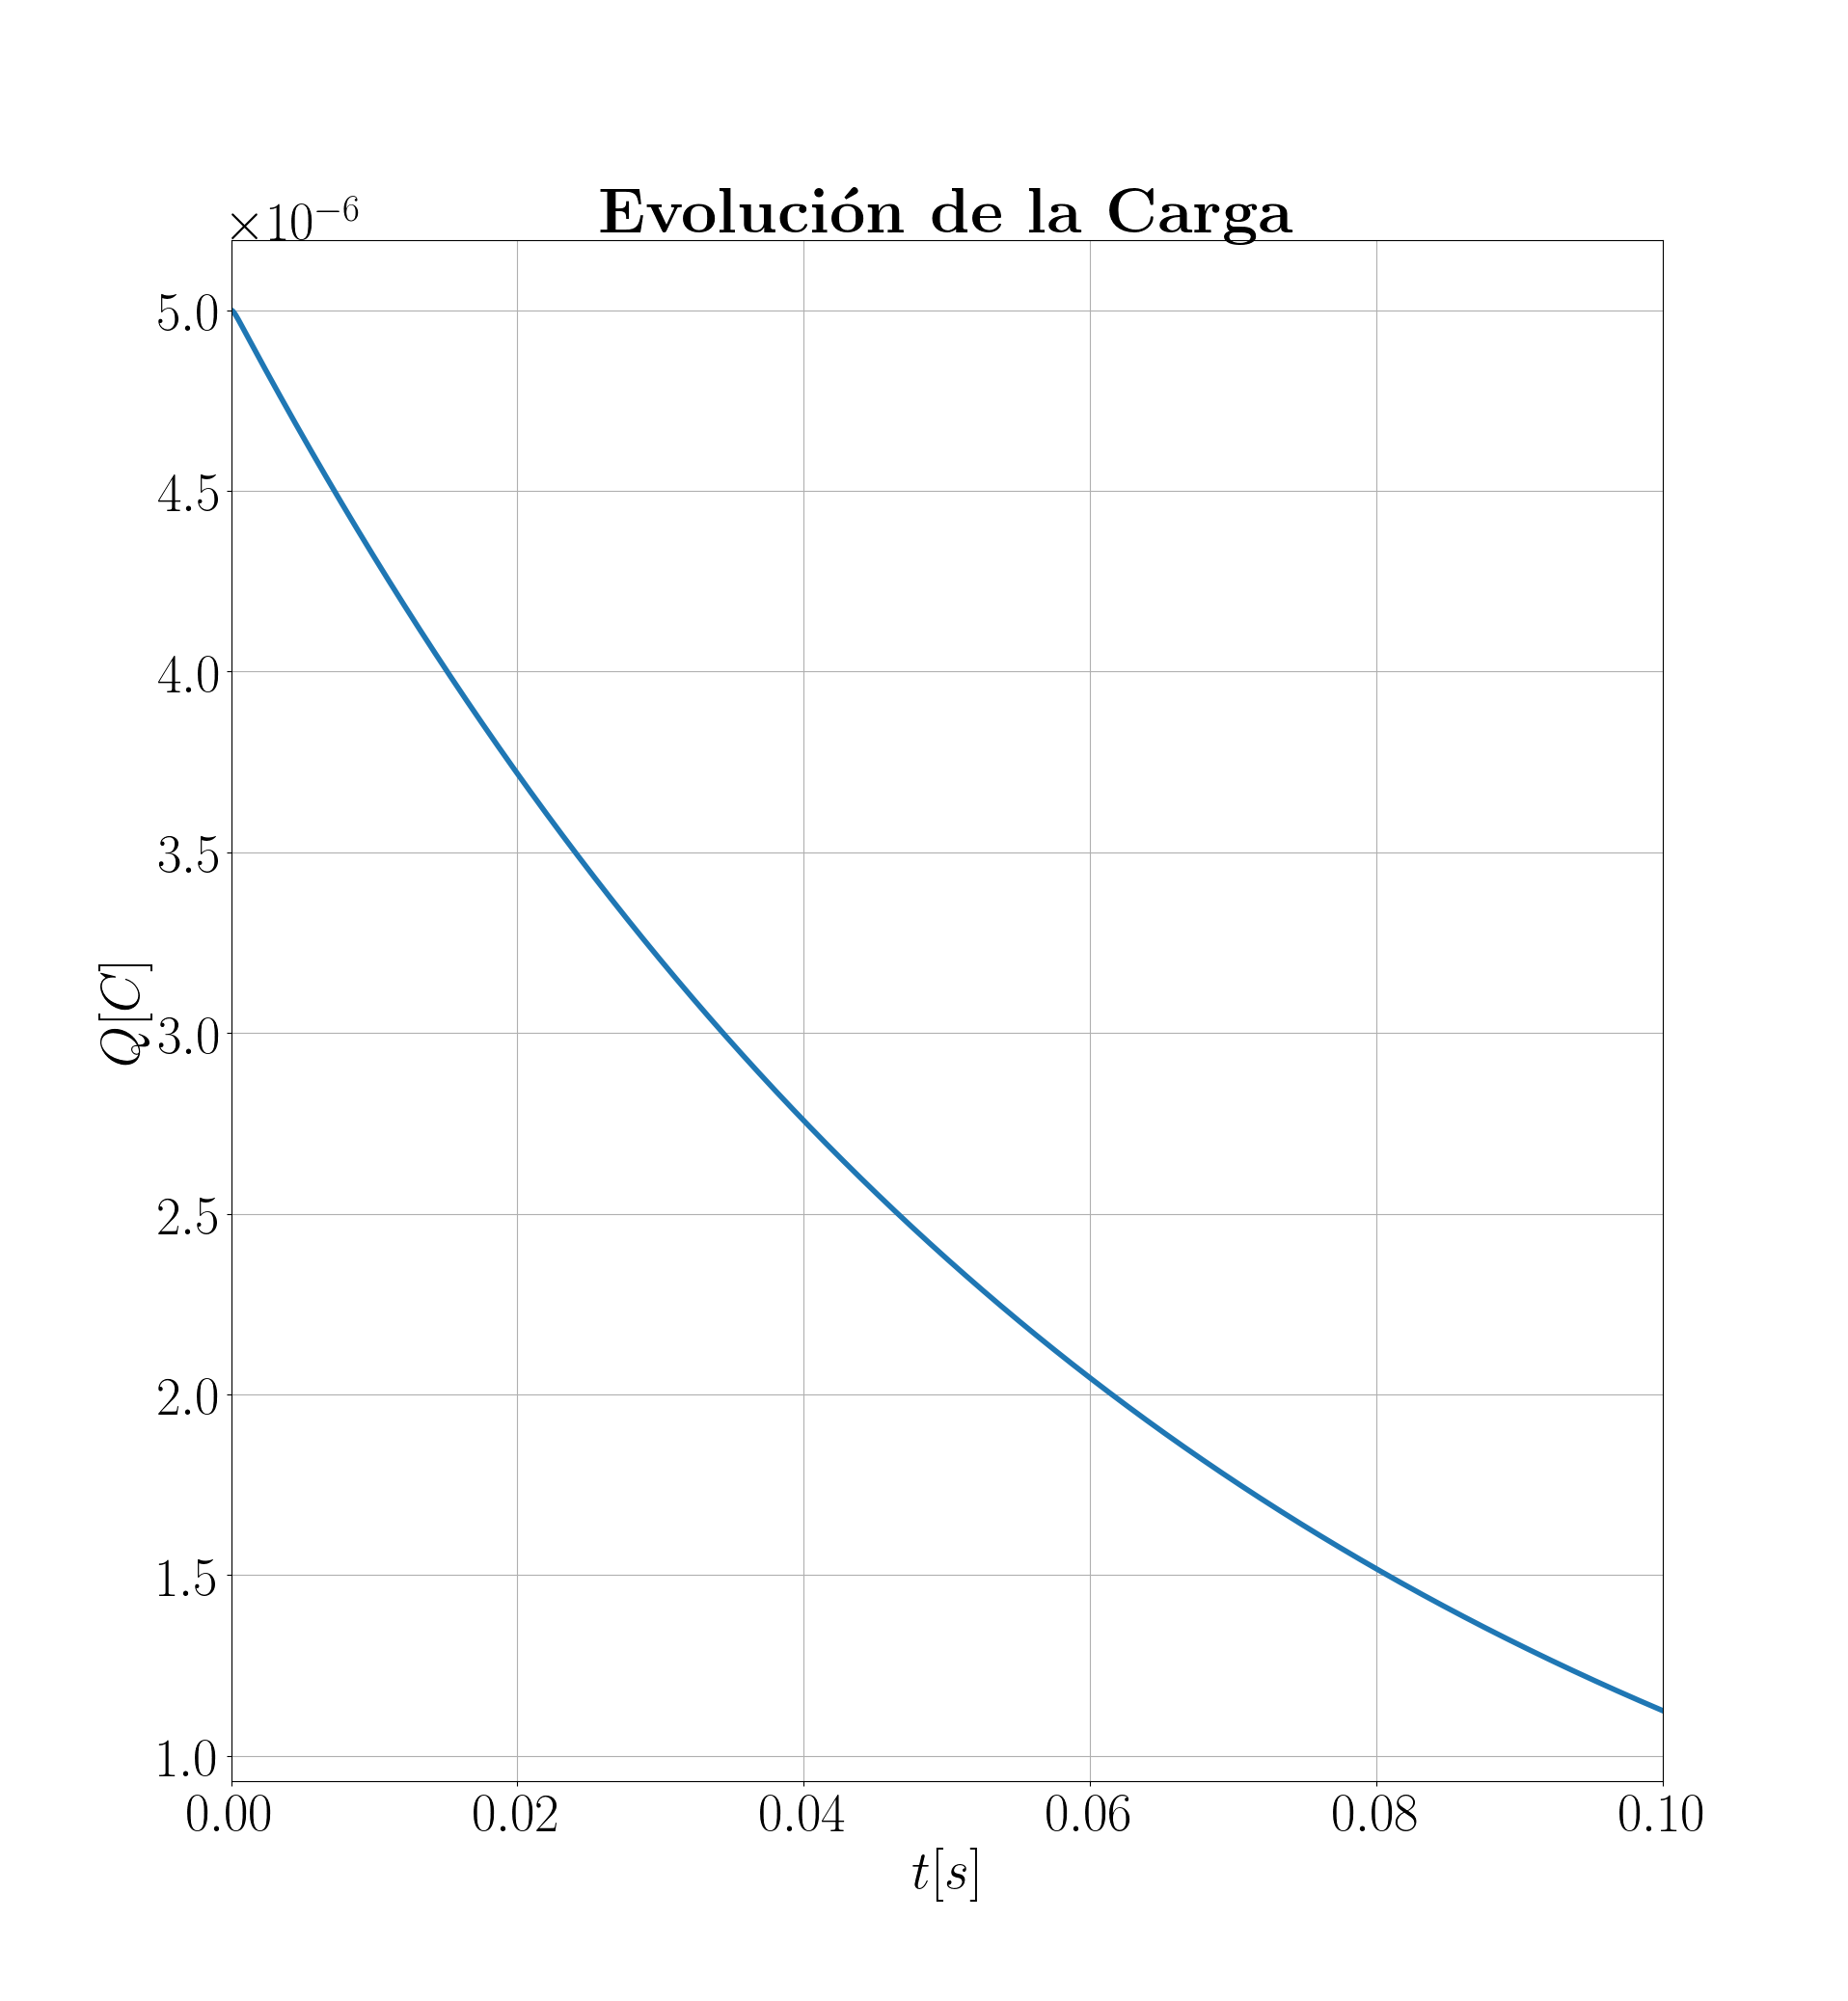
\includegraphics[width=\linewidth,trim={70 70 70 70},clip]{cargasobreamortiguado.png}
    \caption{Evolución de la carga $Q~[C]$ en el caso sobreamortiguado para $R=10 \cdot\sqrt{\frac{4L}{C}}~[\Omega]$.}
    \label{fig:cargasobreamortiguado}
\end{figure}

En esta situación podemos comprobar cómo una excesiva resistencia provoca pérdida de energía tal que ni tan siquiera se puede producir oscilación por lo que se produce una respuesta sobreamortiguada. La pérdida de energía debido a la resistencia provoca que la carga en el condensador no pueda oscilar e invertir la intensidad de la corriente. La solución a la ecuación característica del circuito $RLC$ en este caso da lugar a una corriente resultado de la superposición de dos exponenciales reales que decrecen hasta cero por lo que eventualmente dejará de existir corriente en el circuito y su energía será nula.

\begin{figure}[!htb]
    \centering
    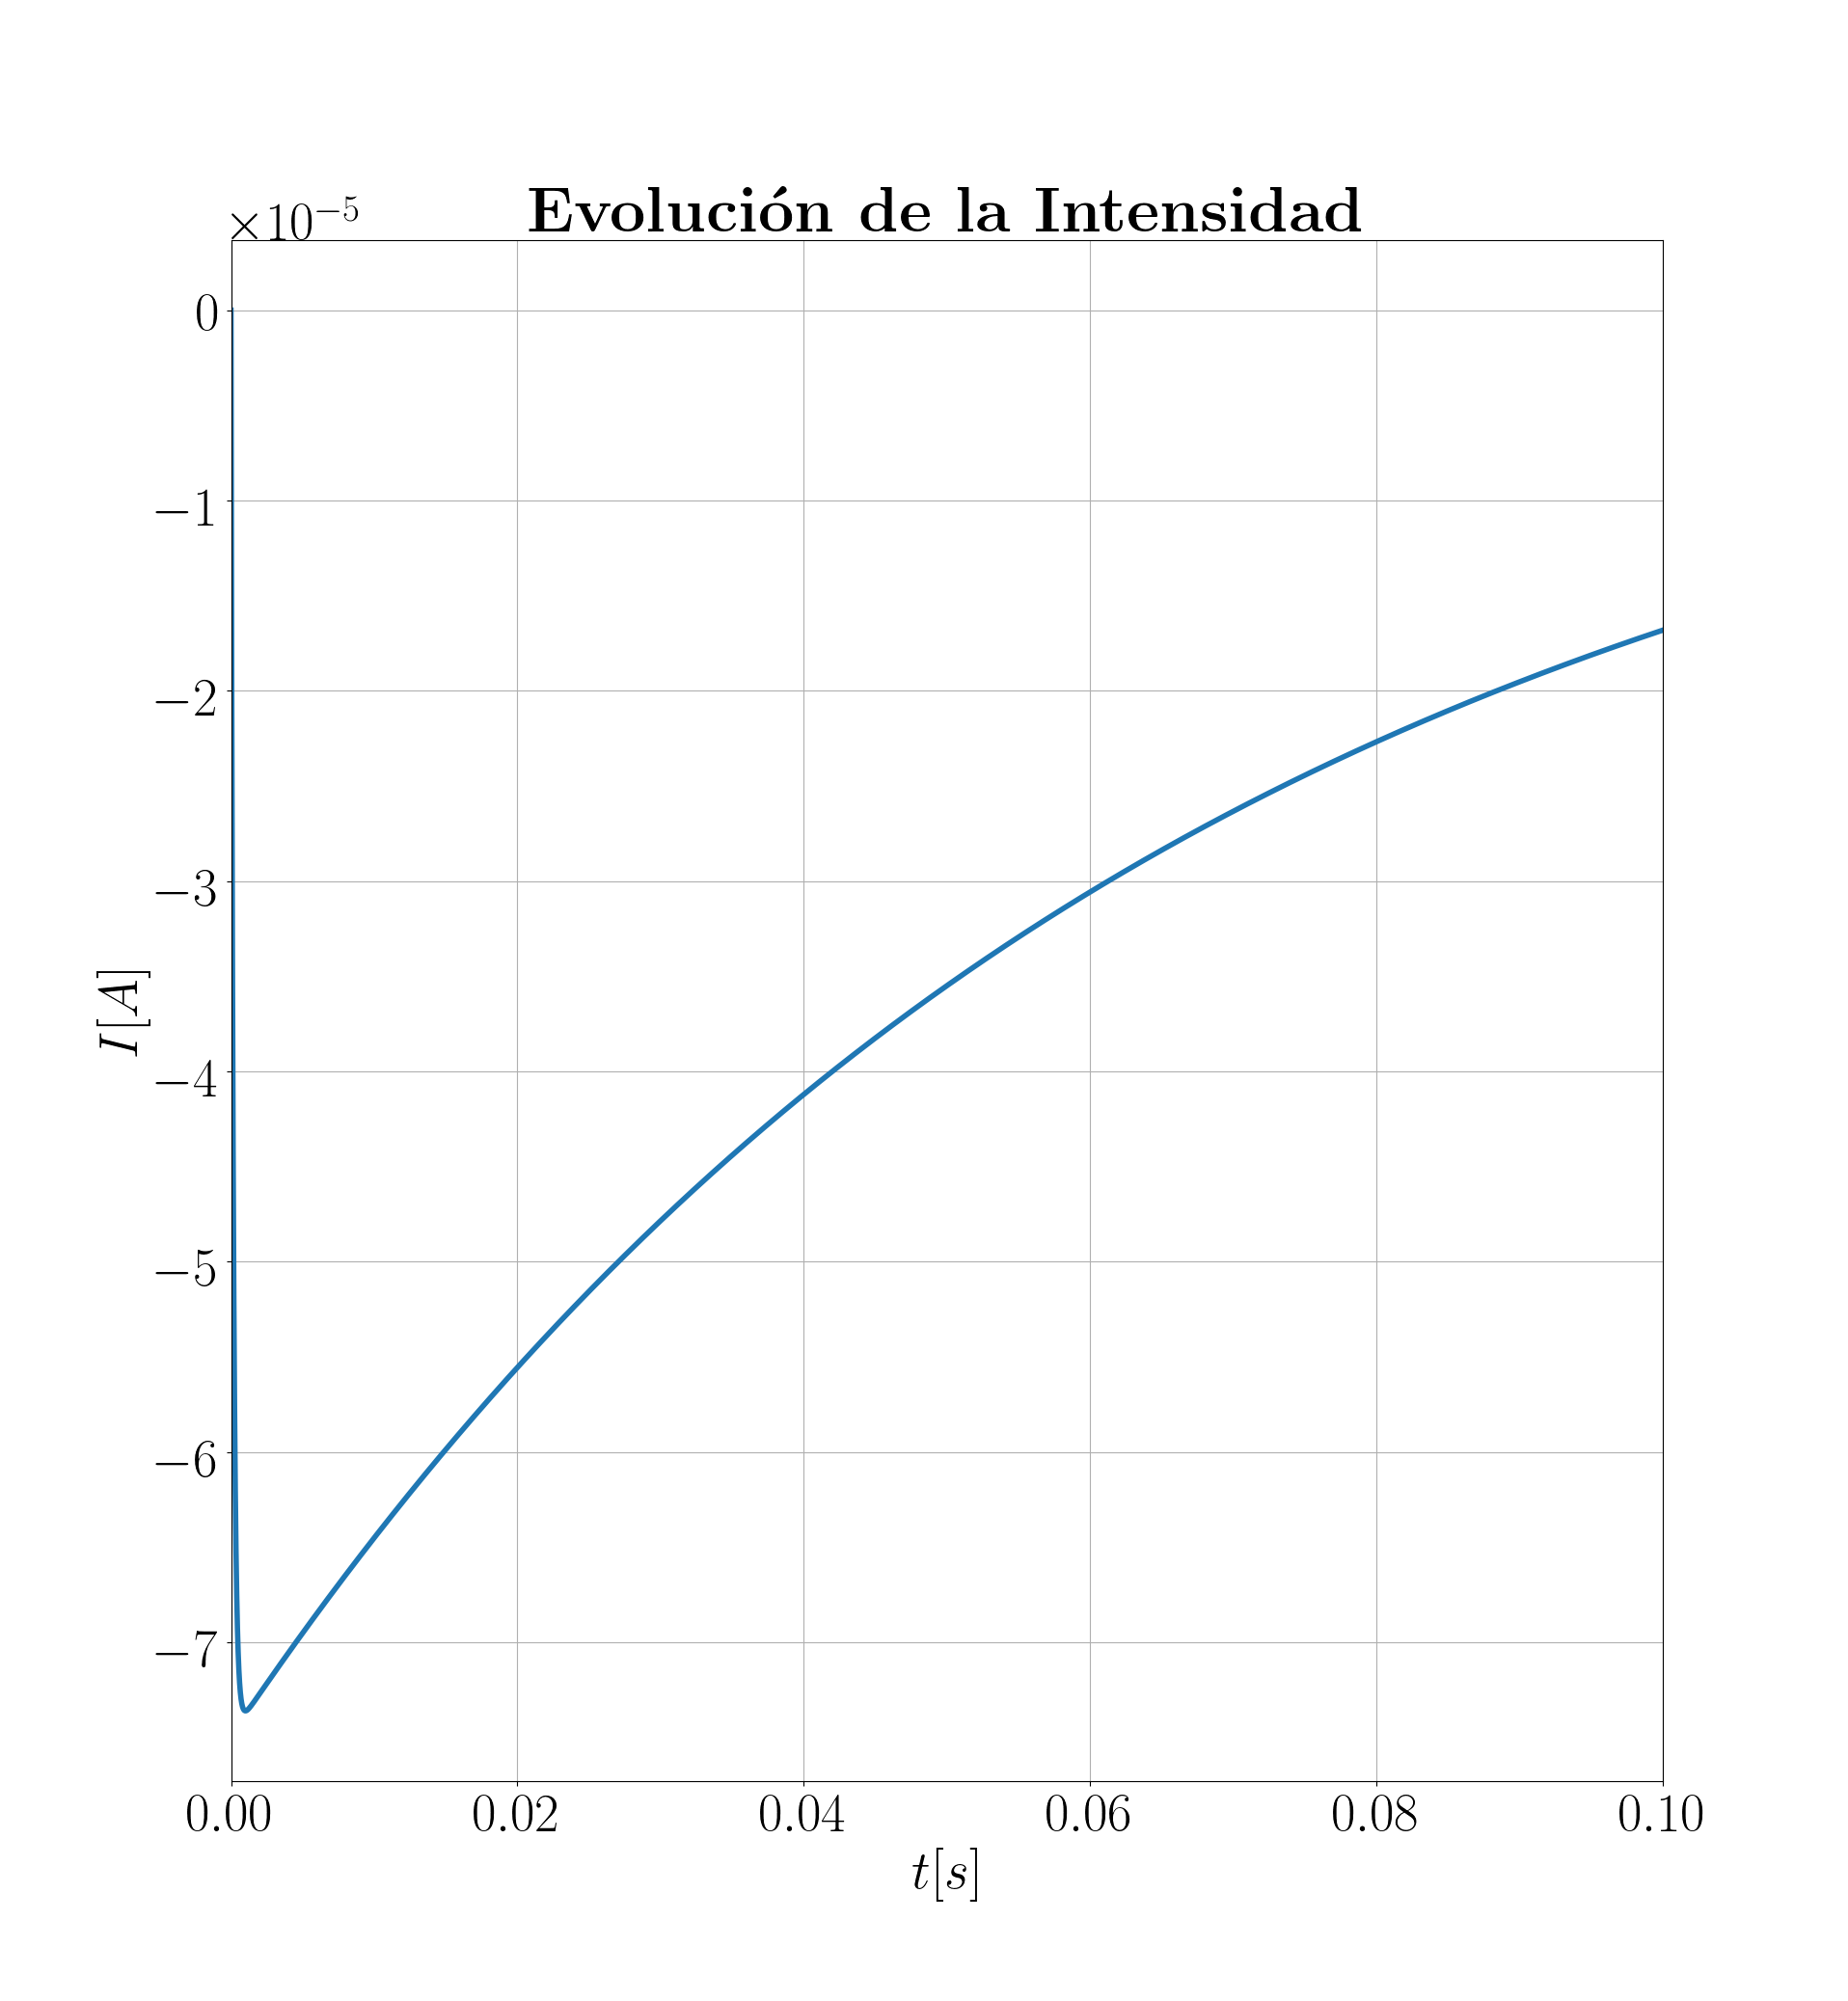
\includegraphics[width=\linewidth,trim={40 70 70 70},clip]{intensidadsobreamortiguado.png}
    \caption{Evolución de la intensidad $I~[A]$ en el caso sobreamortiguado para $R=10 \cdot\sqrt{\frac{4L}{C}}~[\Omega]$.}
    \label{fig:intensidadsobreamortiguado}
\end{figure}

\begin{figure}[!htb]
    \centering
    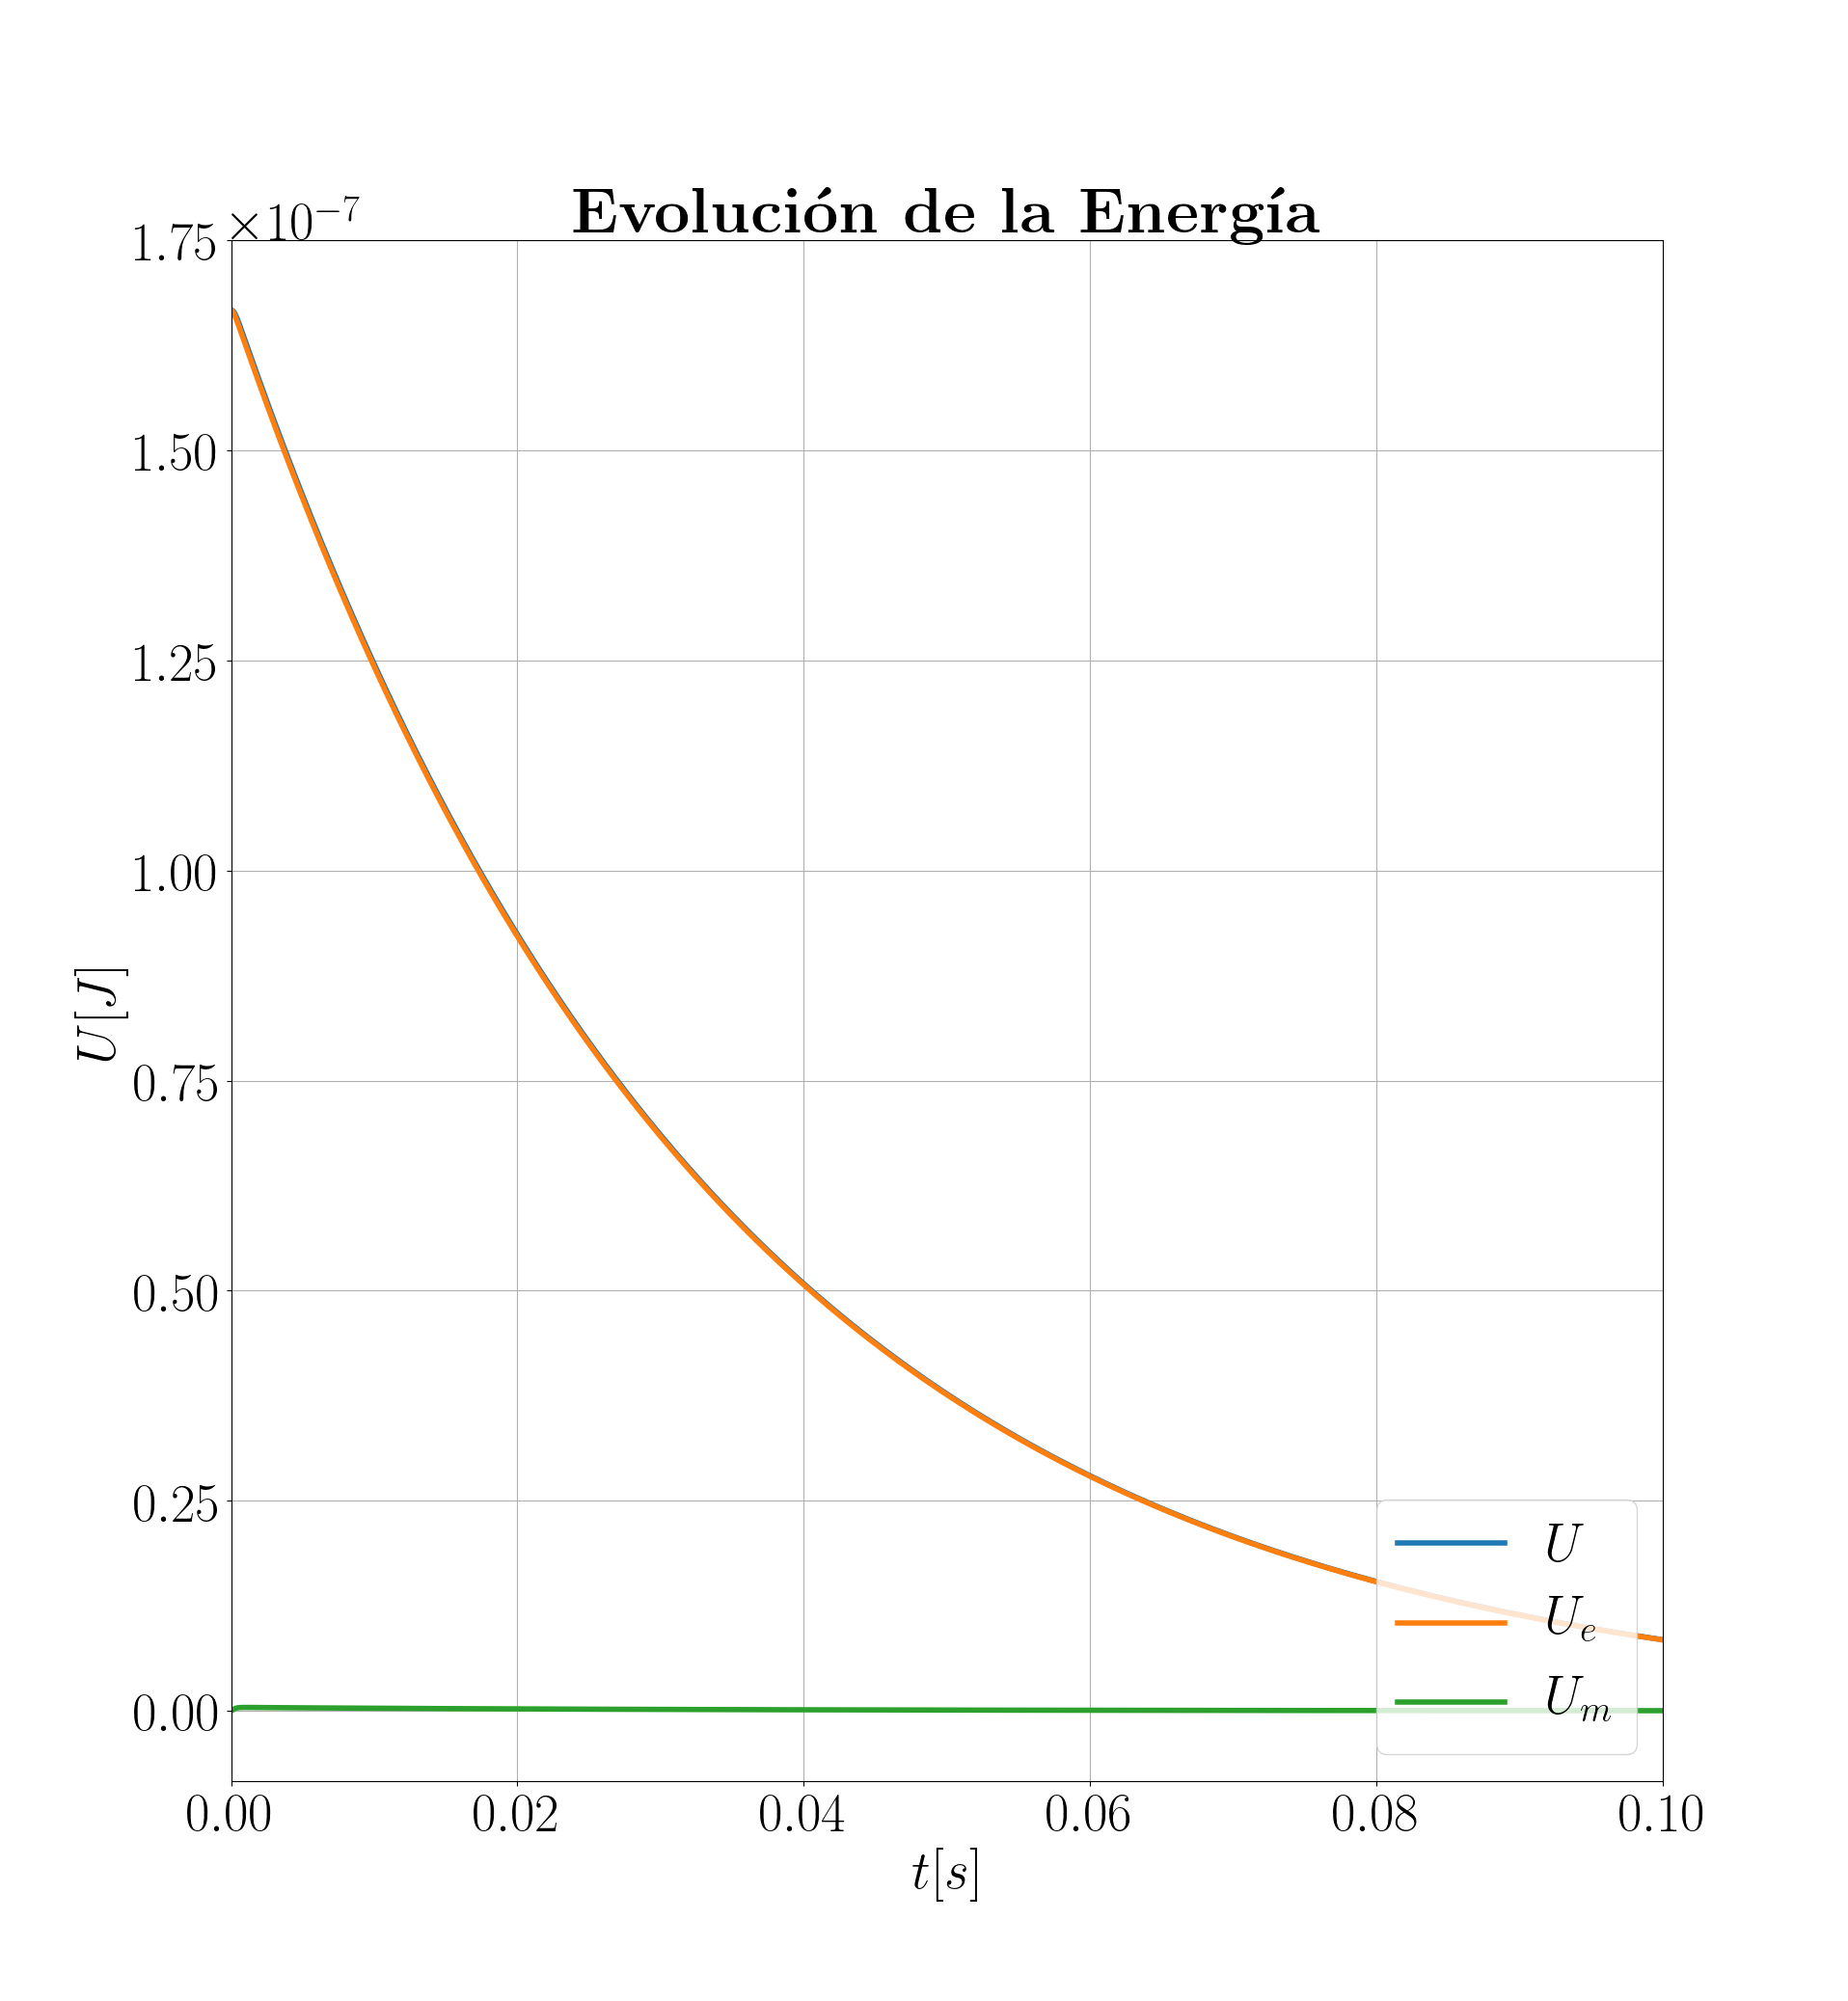
\includegraphics[width=\linewidth,trim={40 70 70 70},clip]{energiasobreamortiguado.png}
    \caption{Evolución de las energías magnética $U_m$, electrostática $U_e$ y total $U$ en el caso sobreamortiguado para $R=10 \cdot\sqrt{\frac{4L}{C}}~[\Omega]$. Nota: la energía total $U$ coincide con la energía electrostática $U_e$.}
    \label{fig:energiasobreamortiguado}
\end{figure}

\clearpage

\subsection{Energía Disipada}

Por último, de forma opcional, se nos plantea calcular la energía disipada en la resistencia conociendo la intensidad (cuyas gráficas se muestran en las Figuras \ref{fig:intensidadsubamortiguado} y \ref{fig:intensidadsobreamortiguado} para los casos subamortiguado y sobreamortiguado respectivamente):

\begin{equation}
U_R = \int_o^\infty I^2(t)R dt~[J]~.
\end{equation}

La implementación que nos permite resolver dicha integral se muestra en el Código \ref{listing:disipada} tal y como hemos desarrollado en el código adjunto a esta práctica.

\bigskip

\begin{code}
    \begin{minted}{python}
ue_ = 0.5 * np.square(z[:, 0]) / C
um_ = 0.5 * L * np.square(z[:, 1])
u_ = ue_ + um_

ur_ = np.zeros_like(u_)
for i in range(len(t)-1):
    ur_[i+1] = ur_[i] + z[i,1] * z[i,1] * R
    \end{minted}
    \caption{Cálculo de la energía disipada.}
    \label{listing:disipada}
\end{code}

Una vez ejecutada dicho cálculo podemos obtener la evolución de la energía disipada en función del tiempo. Las gráficas de dichas evoluciones se muestran en las Figuras \ref{fig:energiadisipadasubamortiguado} y \ref{fig:energiadisipadasobreamortiguado} para los casos subamortiguado y sobreamortiguado respectivamente.

\begin{figure}[!htb]
    \centering
    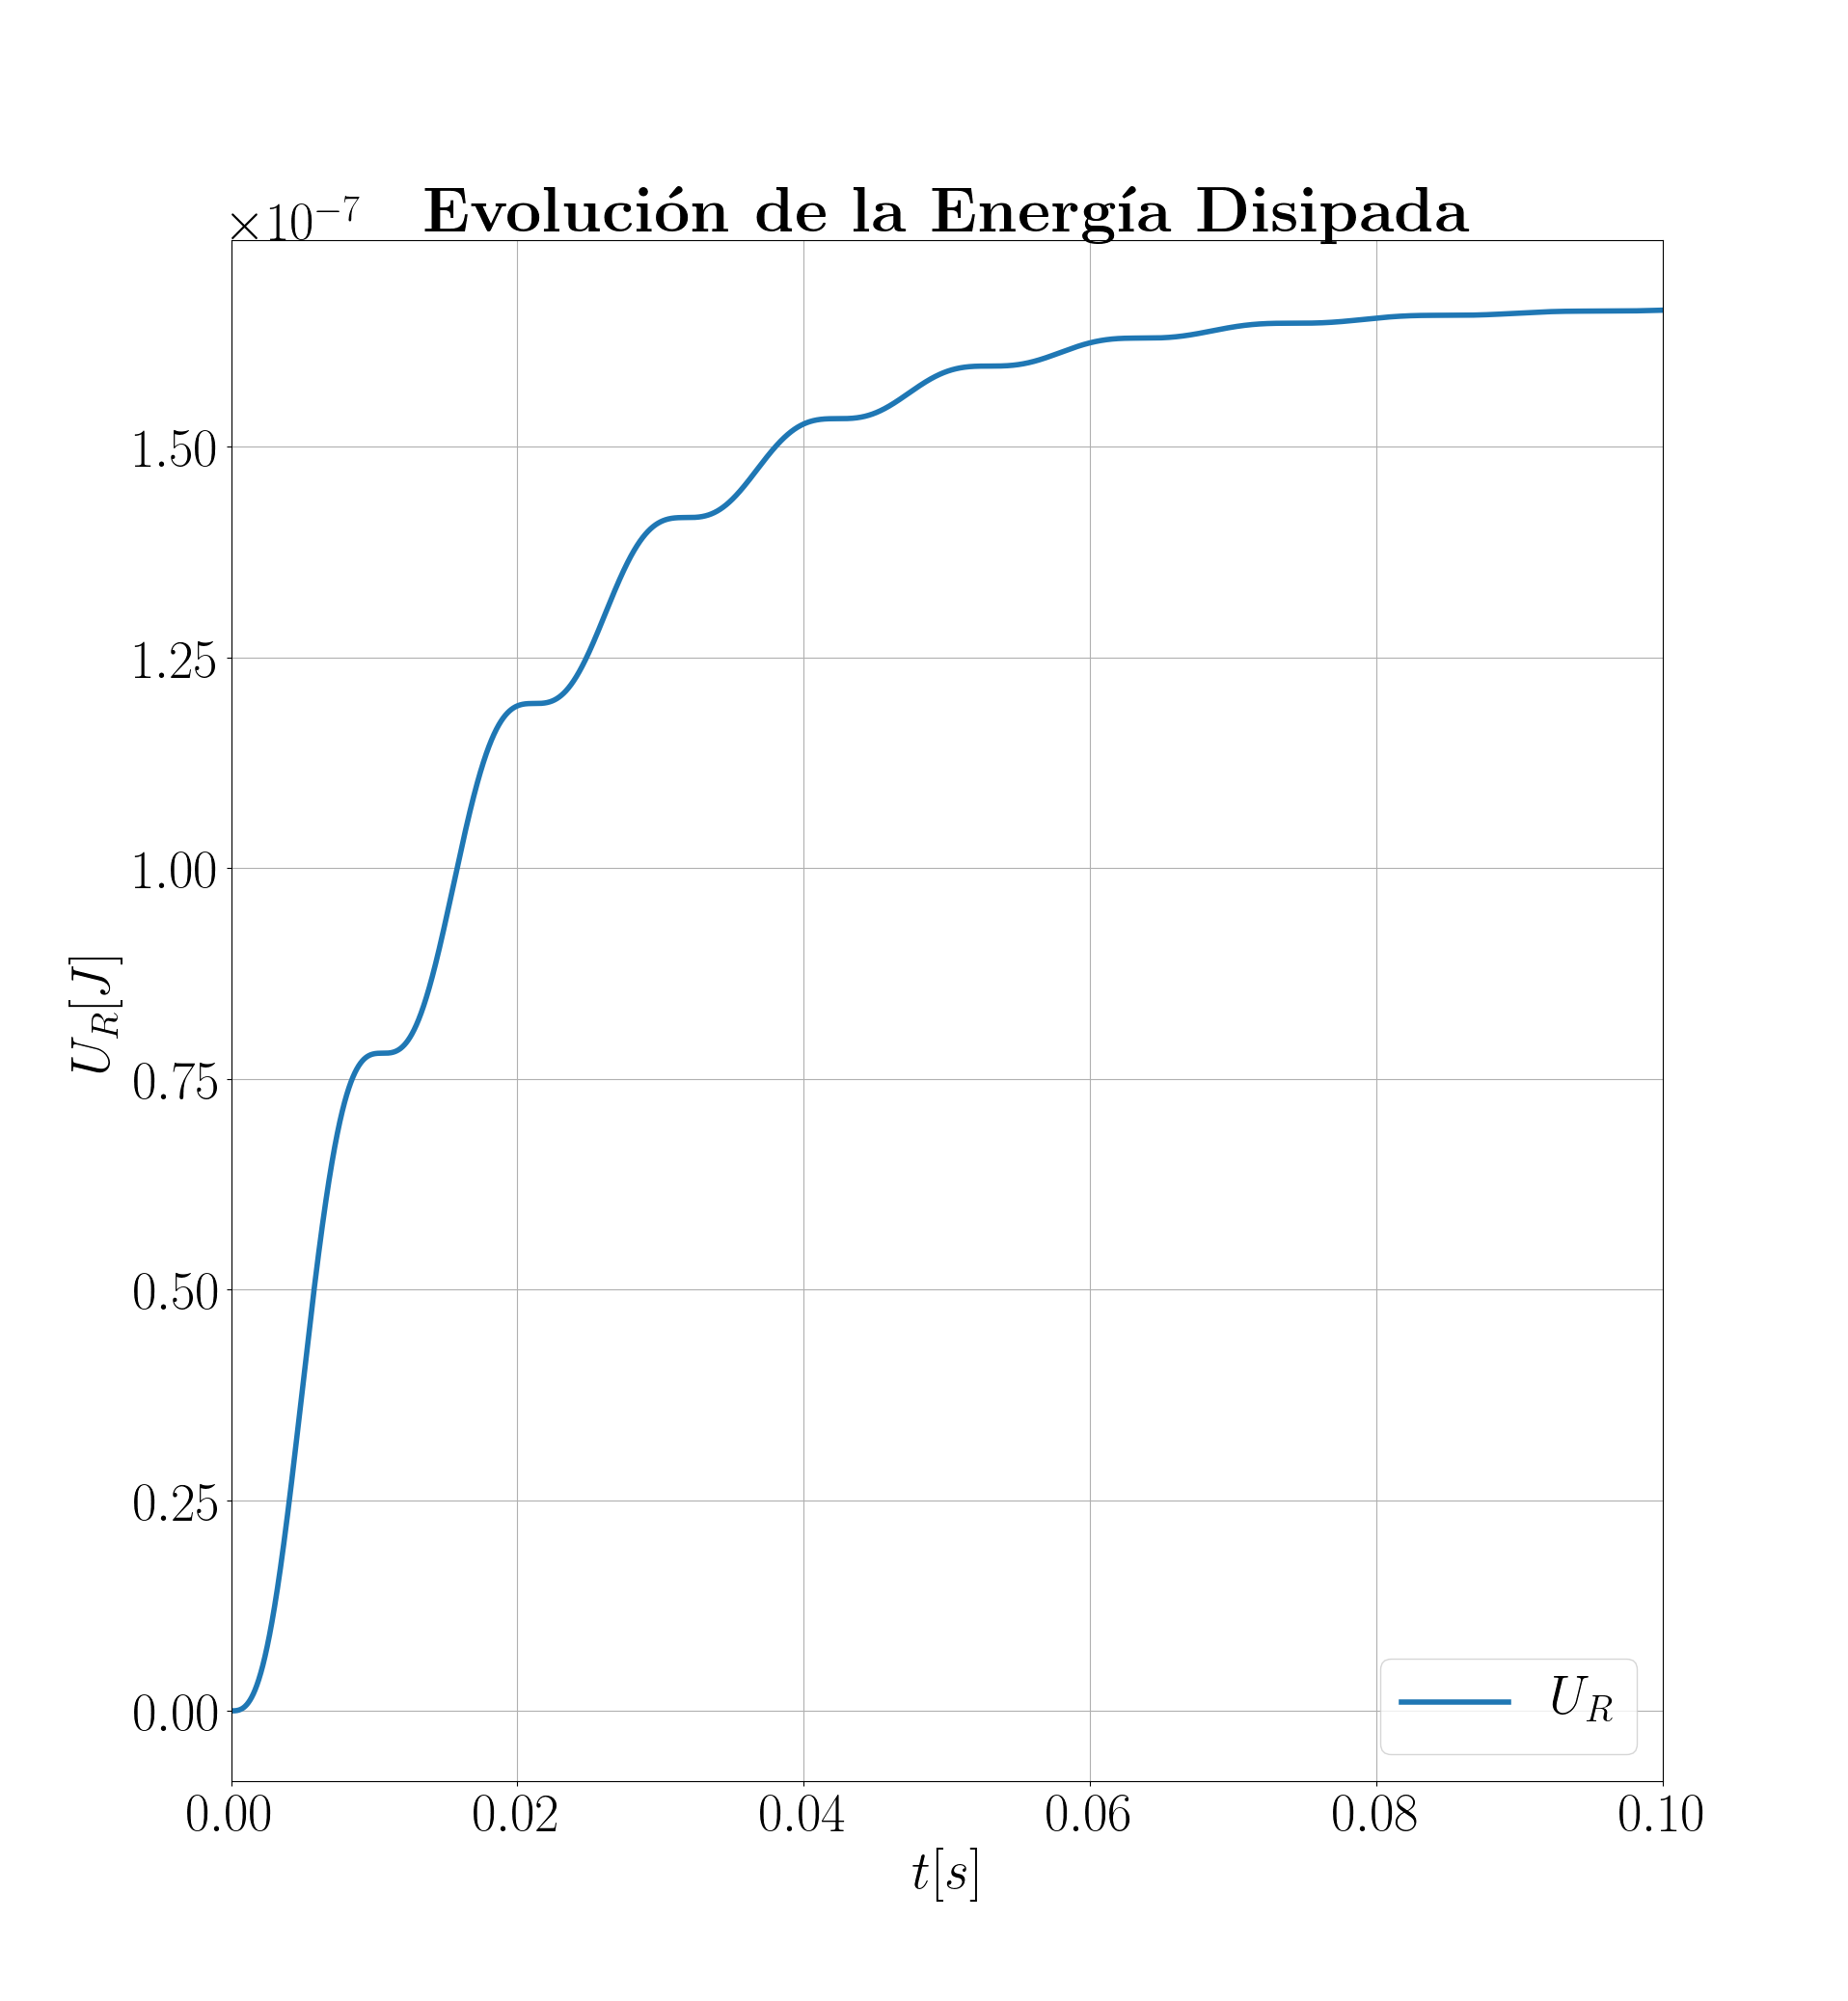
\includegraphics[width=\linewidth,trim={40 70 70 70},clip]{energiadisipadasubamortiguado.png}
    \caption{Evolución de la energía disipada en función del tiempo en el caso subamortiguado para $R=0.1 \cdot\sqrt{\frac{4L}{C}}~[\Omega]$.}
    \label{fig:energiadisipadasubamortiguado}
\end{figure}

\begin{figure}[!htb]
    \centering
    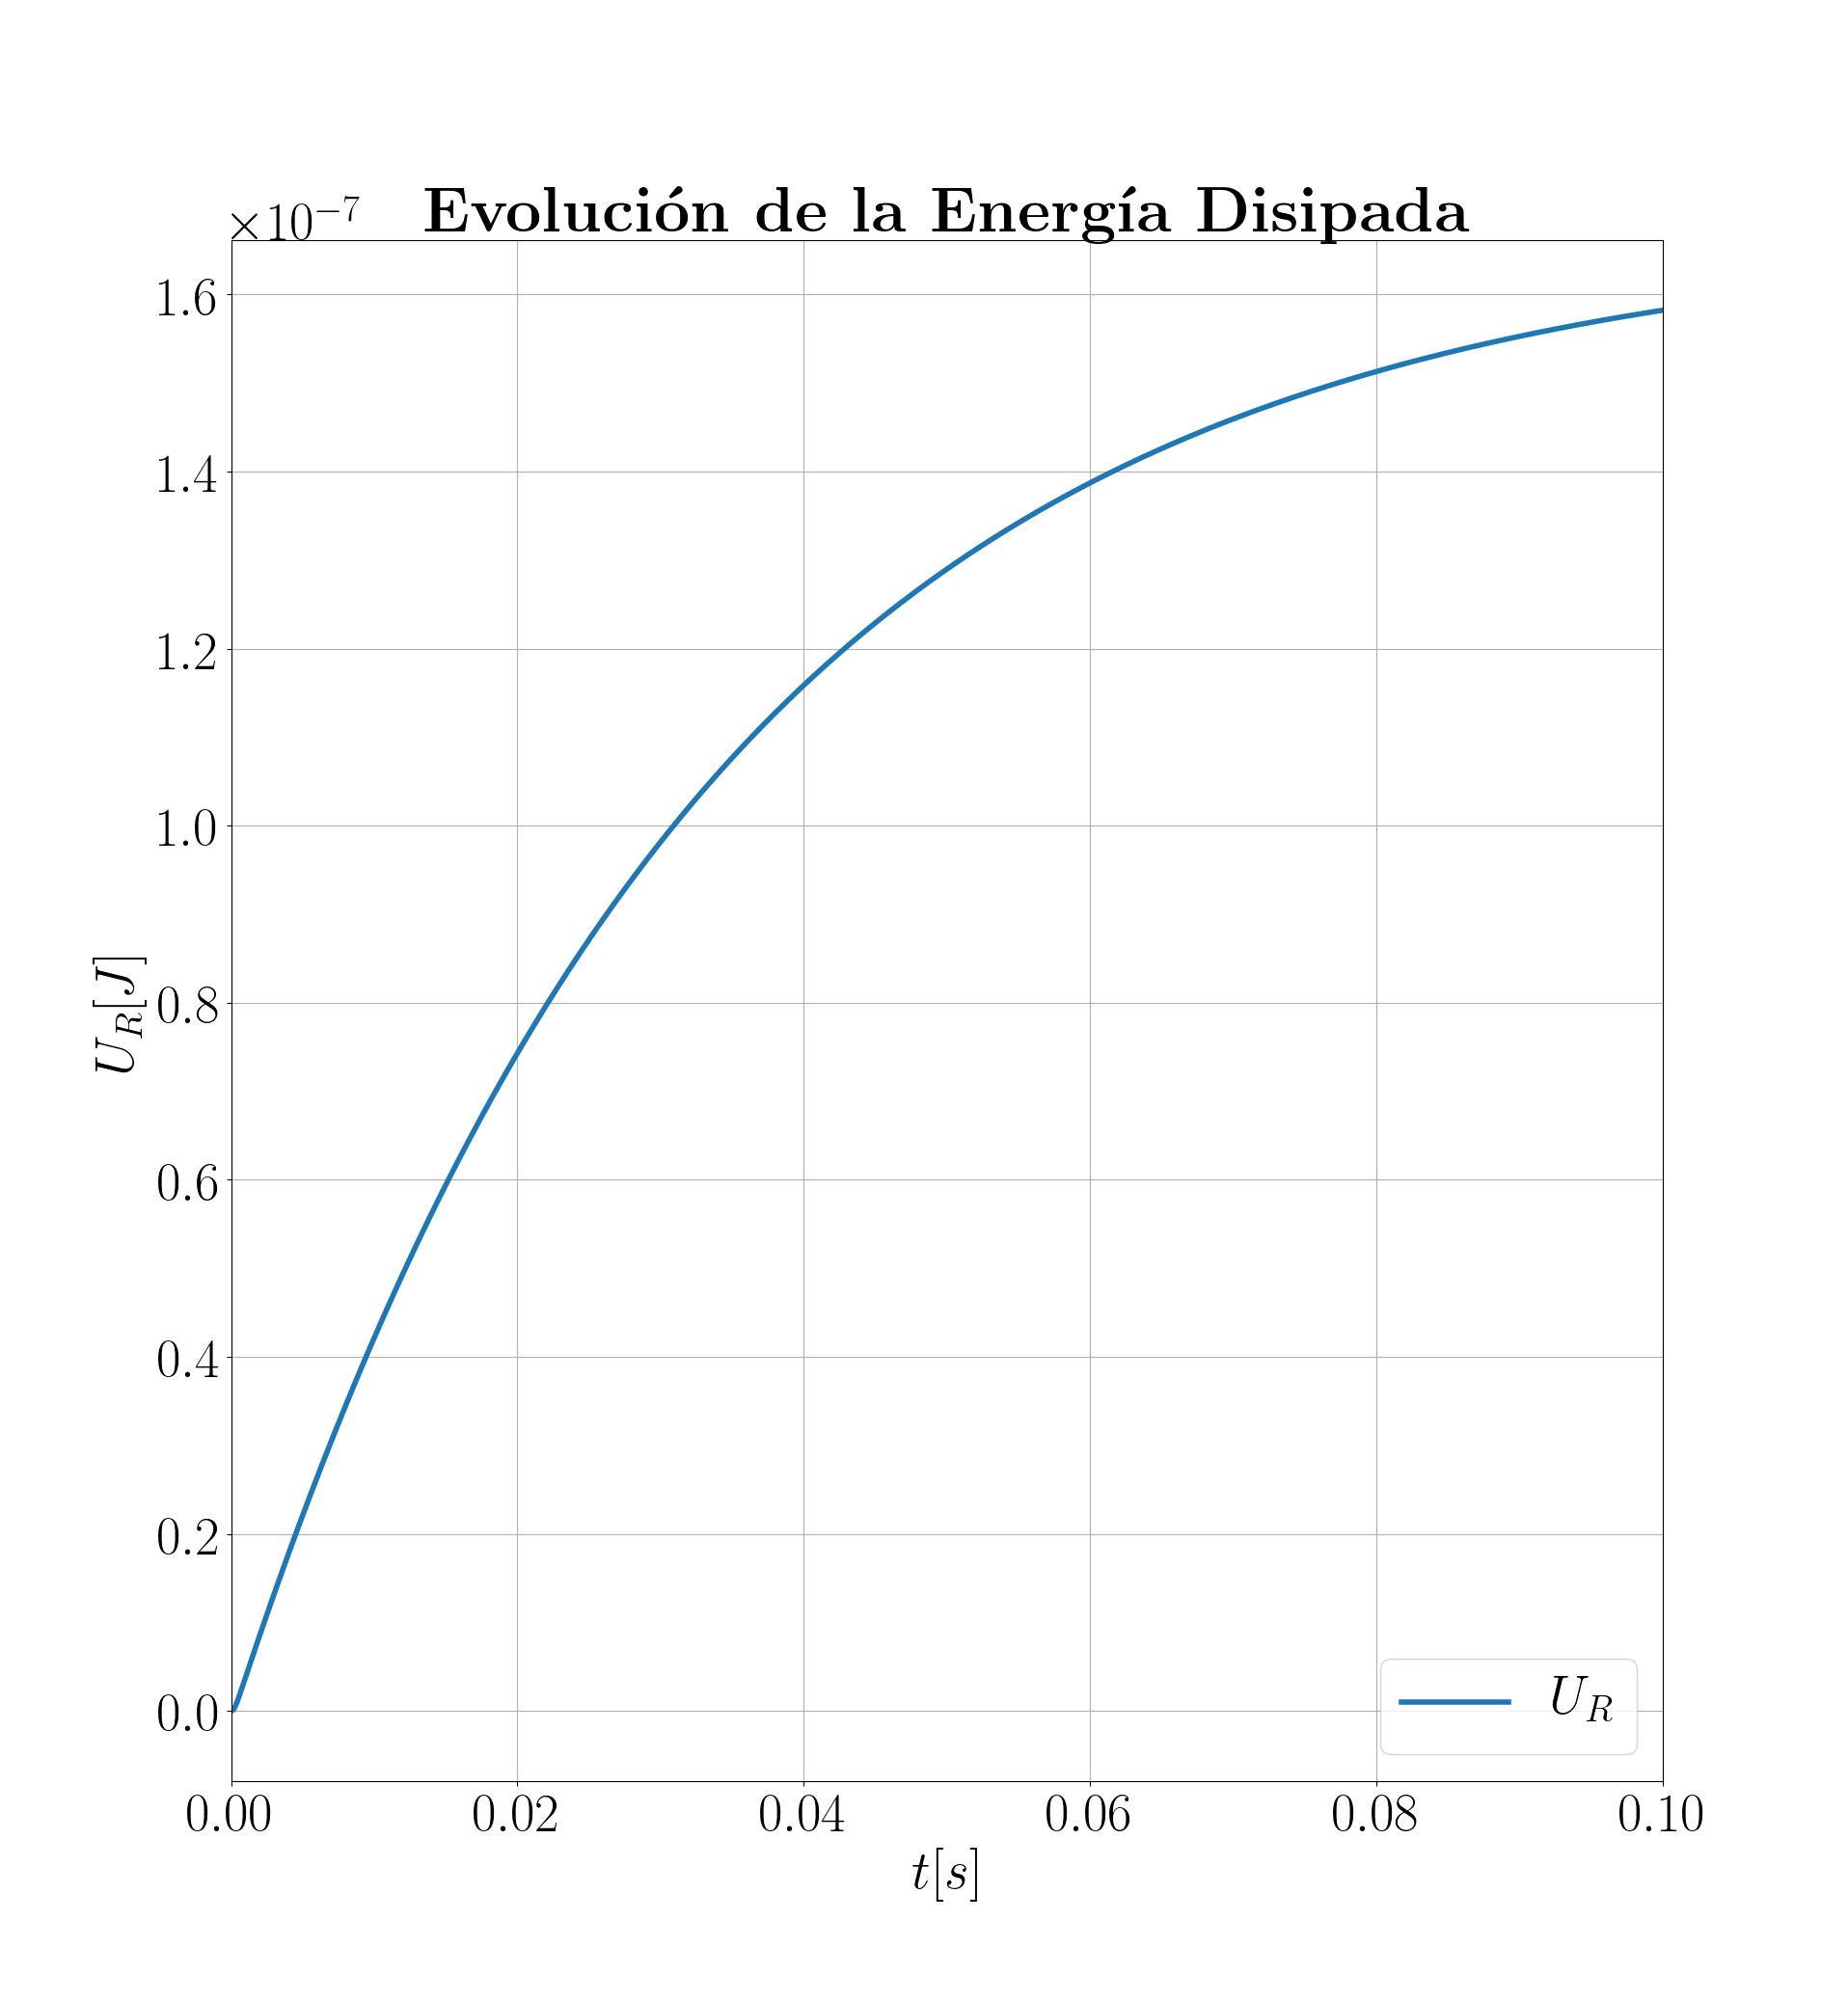
\includegraphics[width=\linewidth,trim={40 70 70 70},clip]{energiadisipadasobreamortiguado.png}
    \caption{Evolución de la energía disipada en función del tiempo en el caso sobreamortiguado para $R=10 \cdot\sqrt{\frac{4L}{C}}~[\Omega]$.}
    \label{fig:energiadisipadasobreamortiguado}
\end{figure}

Como podemos observar, el valor final de $U_R$ (tras un tiempo suficiente para que la intensidad se vea reducida a cero) converge con el valor inicial de $U_e$ que tenía el condensador inicialmente en ambos casos (ver Figuras \ref{fig:energiasubamortiguado} y \ref{fig:energiasobreamortiguado}): aproximadamente $1.66\cdot 10^{-7}~[J]$ en ambos casos.

\newpage

\section{Circuito RLC en Serie con Generador}
\label{sec:rlccongenerador}

En esta segunda sección estudiaremos el sistema mostrado en la Figura \ref{fig:rlcgen}. En este caso disponemos de un generador de voltaje alterno en serie con una disposición similar al circuito anterior: un condensador incialmente descargado, una resistencia y una bobina. El generador produce un voltaje alterno del tipo $V(t) = V_0 \cos{\omega t}$.

\begin{figure}[!htb]
    \centering
    \begin{circuitikz}
        \draw[ very thick](5,3)-- +(30:0.46);
        \draw (0,0)
          to[C=\(C\),i=$I$] (0,3) % The voltage source
          to[R=\(R\),i=$I$] (5,3) % The resistor
          to[short,-o](5,3)
          (5.5,3)to[short,o-](6,3)
          to[L=\(L\),i=$I$] (6,0) % The inductor
          to[sinusoidal current source] (3, 0)
          to (0,0); %Inductor One
        \end{circuitikz}
        \medskip
        \caption{Circuito RLC en serie con generador.}
        \label{fig:rlcgen}
\end{figure}

De forma teórica, podemos expresar la ecuación que controla el sistema como la equivalente a la de un oscilador armónico amortiguado y forzado:

\begin{equation}
L\frac{d^2Q}{dt^2} + R\frac{dQ}{dt} + \frac{1}{C}Q = V_s = V_0\cos{\omega t}
\end{equation}

\clearpage

\subsection{Estudio Teórico Mediante Método de Fasores}
\label{subsec:estudioteorico}

Sabemos que el voltaje del circuito se puede expresar como

\begin{equation}
V_s = IZ~[V]~,
\end{equation}

siendo $Z$ la impedancia del circuito que posee tres componentes: la impedancia resistiva $R$, la impedancia capacitiva $X_C$ y la impedancia inductiva o reactancia $X_L$. Por lo tanto, el voltaje posee tres componentes:

\begin{equation}
V_R = IR~[V]~,
\end{equation}
\begin{equation}
V_C = IX_C = I \frac{-i}{\omega C}~[V]~,
\end{equation}
\begin{equation}
V_L = IX_L = Ii\omega L~[V]~,
\end{equation}

así pues, el voltaje se puede expresar como

\begin{equation}
\vec{V}_L + \vec{V}_C + \vec{V}_R = (V_R)\hat{u}_x + (V_L - V_C)\hat{u}_y~[V]~.
\end{equation}

El módulo de dicho vector (con componentes imaginaria y real) es la impedancia del circuito $Z$ multiplicada por la corriente $I$, el ángulo $\delta$ que forma con el eje horizontal es el desfase entre la corriente y el voltaje aplicado.

\begin{equation}
|\vec{V}_L + \vec{V}_C + \vec{V}_R| = \sqrt{V_R^2 + (V_L - V_C)^2}
\end{equation}

\begin{equation}
|\vec{V}_L + \vec{V}_C + \vec{V}_R| = \sqrt{(IR)^2 + (I(X_L - X_C))^2}
\end{equation}

\begin{equation}
\mathcal{E}_0 = IZ = I\sqrt{R^2 + (\omega L - \frac{1}{\omega C})^2}
\end{equation}

Así pues, podemos determinar el valor de la intensidad como
\begin{equation}
I = \frac{V_s}{Z} = \frac{V_s}{\sqrt{R^2 + (\omega L - \frac{1}{\omega C})^2}}~[A]~,
\end{equation}
\begin{equation}
I(t) = Io \cdot \cos{(\omega t - \delta)}~[1]~,
\end{equation}

siendo $I_0 = V_0 / Z$ e $I_{ef}=I/\sqrt{2}$.

El desfase entre el volataje y la corriente se puede calcular a partir del ángulo $\delta$ como

\begin{equation}
\tan{\delta} = \frac{|X_L - X_C|}{R}~,
\end{equation}
\begin{equation}
\delta = \arctan{(\frac{\omega L - \frac{1}{\omega C}}{R})}~[rad]~.
\end{equation}

Si $\delta > 0$ significa que la corriente adelanta a la tensión y de lo contrario le tensión adelanta a la corriente.

Conociendo los fundamentos teóricos mediante el método de los fasores podemos calcular, antes de confirmarlos experimentalmente, los valores tanto de la corriente eficaz del circuito como del desfase. Los valores que utilizaremos para este propósito para la simulación se encuentran en el Código \ref{listing:datos_rlccongen} y han sido escogidos siguiendo las restricciones indicadas por el enunciado de la práctica.

\bigskip
\newpage

\begin{code}
    \begin{minted}{python}
        R=300 # Resistencia
        C=75.0e-6  # Condensador
        L=0.30 # Bobina
        Vef=165 # Tension eficaz
        f=75 # Frecuencia
    \end{minted}
    \caption{Datos de simulación para estudio de dinámica de circuito RLC con generador.}
    \label{listing:datos_rlccongen}
\end{code}

La impedancia del circuito es

\begin{equation}
Z = \sqrt{R^2 + (\omega L - \frac{1}{\omega C})^2}
\end{equation}
\begin{equation}
Z=\sqrt{300^2 + (2\pi\cdot 75\cdot 0.30 - \frac{1}{2\pi\cdot 75\cdot 75\cdot 10^{-6}})^2}
\end{equation}
\begin{equation}
Z = 320.60
\end{equation}

El valor eficaz de la corriente es

\begin{equation}
I_{ef} = \frac{I_0}{\sqrt{2}} = \frac{V_{ef}\sqrt{2}}{Z\sqrt{2}} = \frac{165.00}{320.60} = 0.51~[A]~,
\end{equation}

y por lo tanto, su intensidad inicial es

\begin{equation}
I_0 = I_{ef} \sqrt{2} = 0.51 \sqrt{2} = 0.72~[A]~.
\end{equation}

El desfase es

\begin{equation}
\delta = \arctan{\frac{2 \pi \cdot 75.00 \cdot 0.30 - \frac{1}{2 \pi \cdot 75.00 \cdot 75.00\cdot 10^{-6}}}{300}}~.
\end{equation}

\begin{equation}
\delta = 0.38~[rad] = 21.60~[deg]
\end{equation}

Así pues, la intensidad es $I(t) = 0.72\cdot cos(\omega t - 0.38)~[A]$ y dado que $\delta > 0$ adelanta a la tensión.

\begin{figure}[!htb]
    \centering
    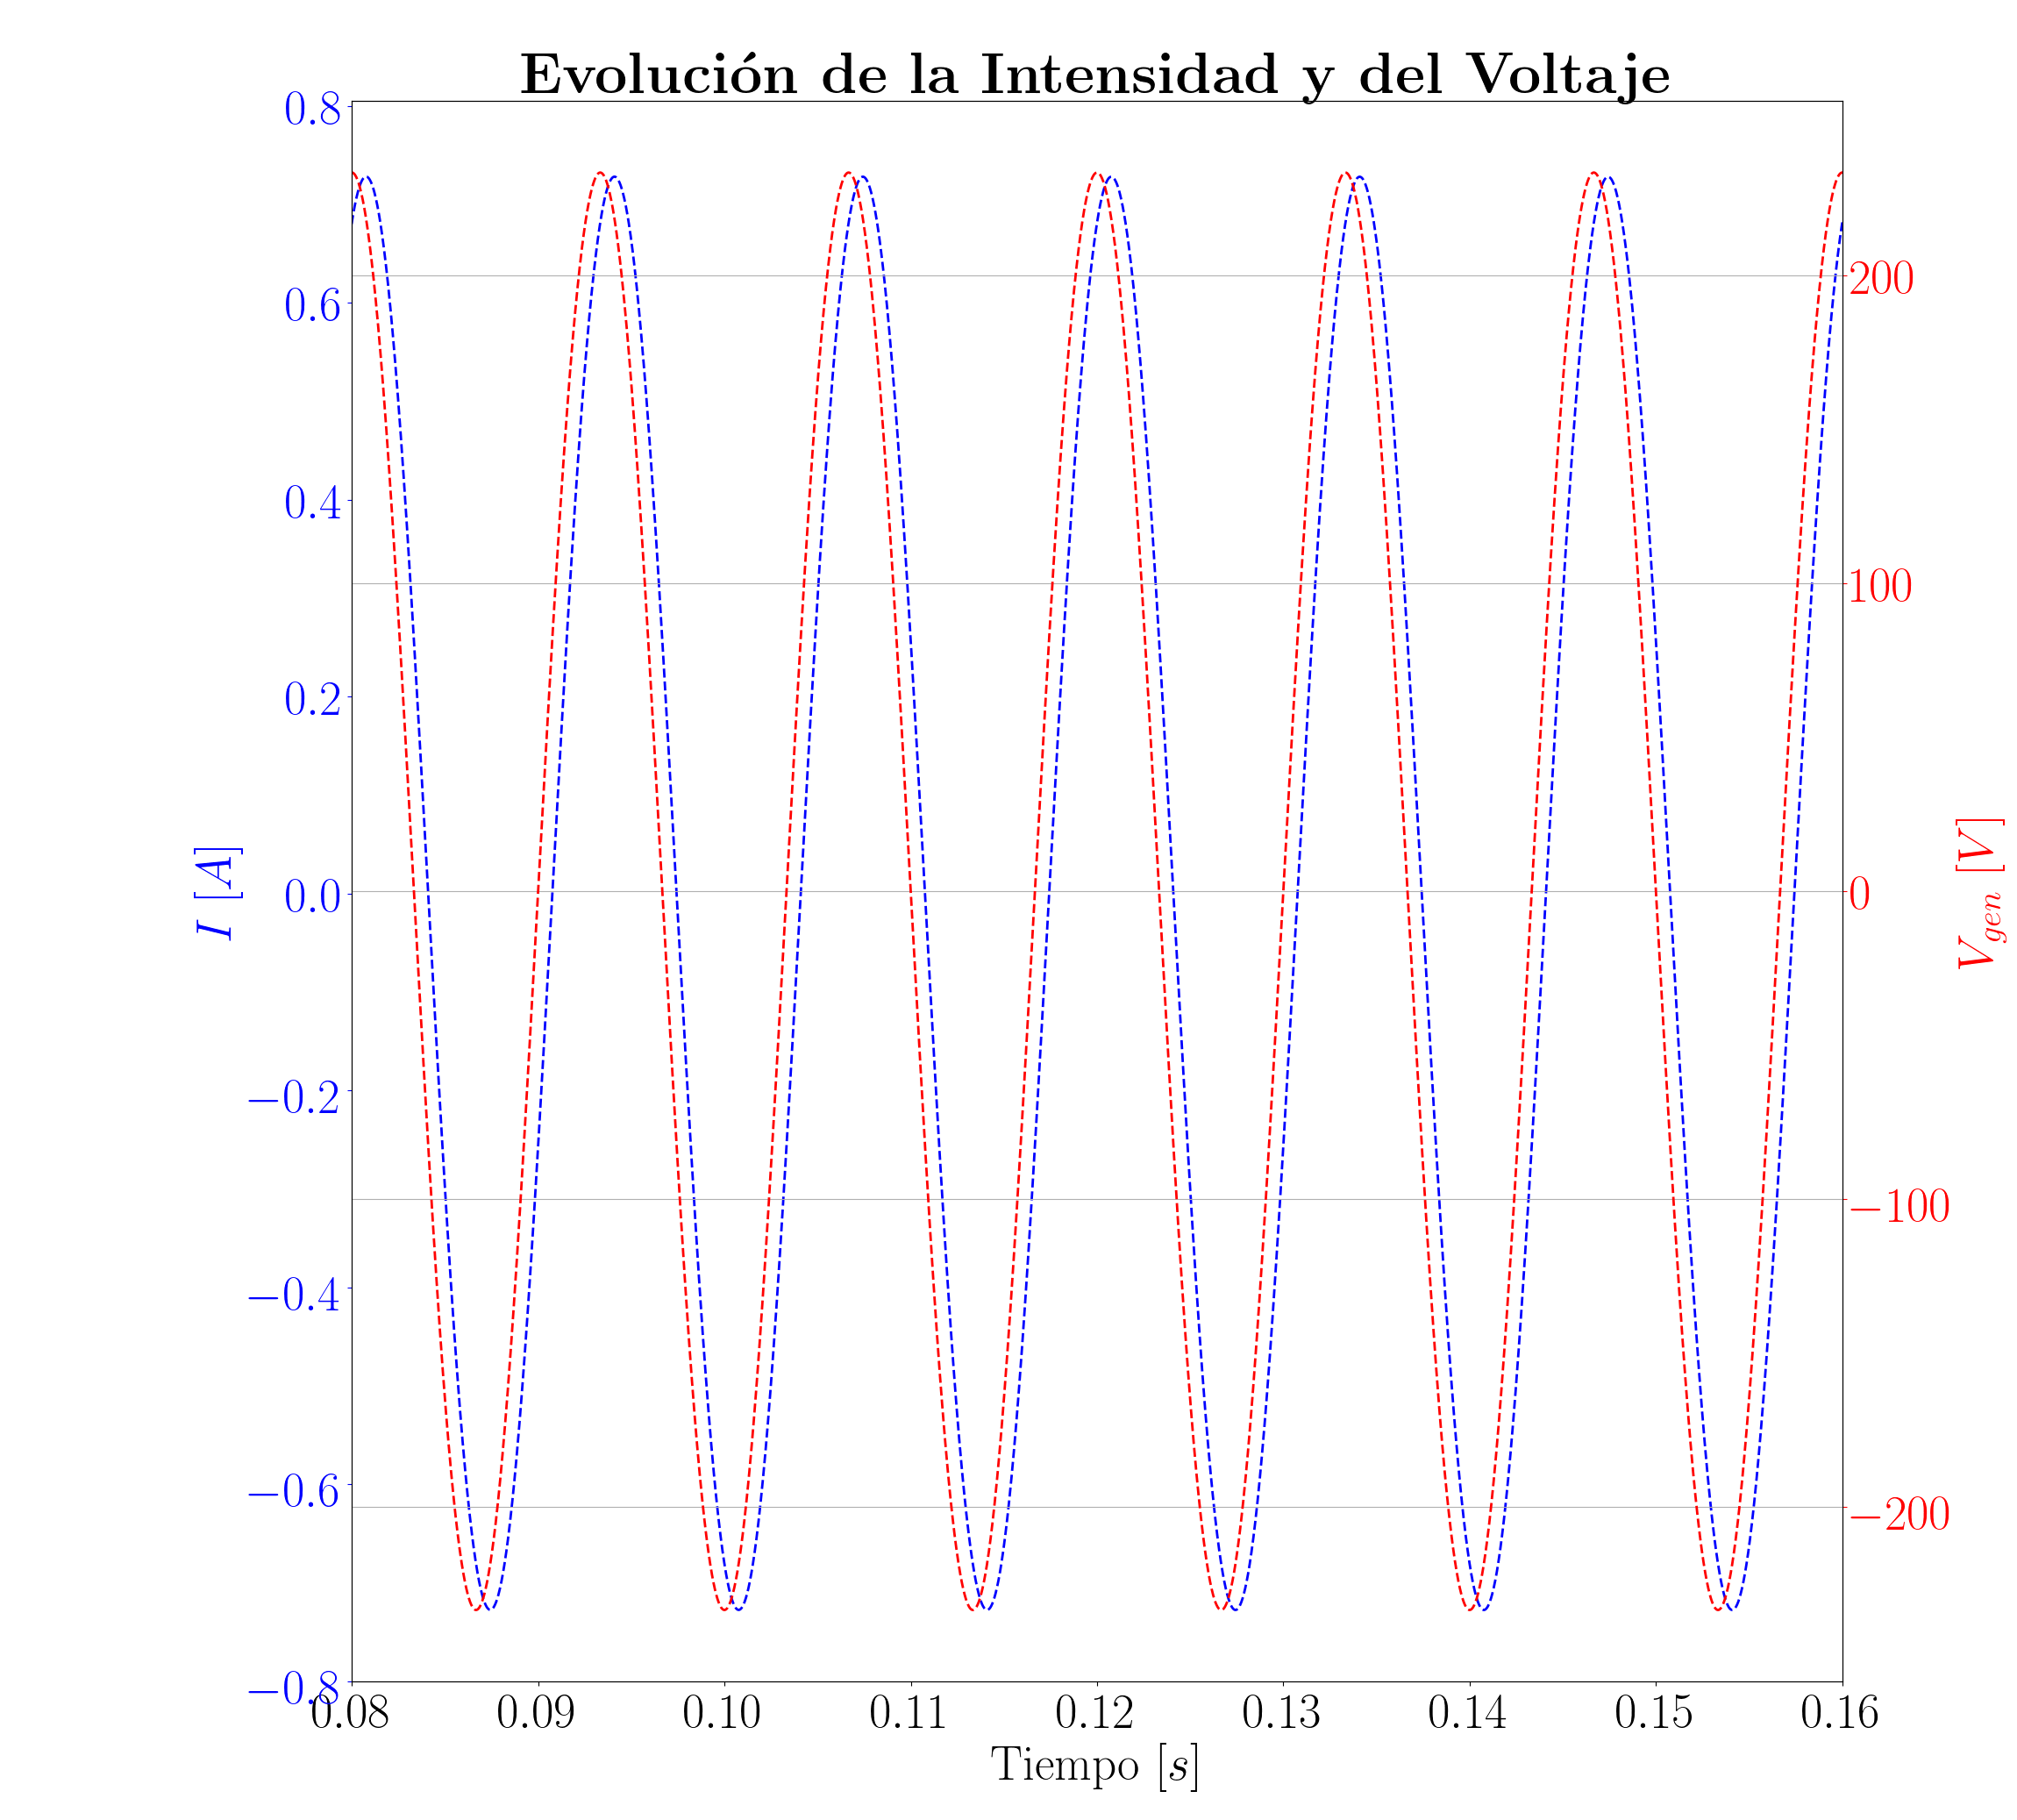
\includegraphics[width=\linewidth,trim={120 0 0 40},clip]{congenintensidadvoltaje.png}
    \caption{Evolución de la intensidad y del voltaje para el circuito RLC con generador.}
    \label{fig:congenintensidadvoltaje}
\end{figure}

Como podemos observar en la gráfica mostrada en la Figura \ref{fig:congenintensidadvoltaje}, la intensidad toma un valor máximo $I_0 \simeq 0.71$ que coincide (con el margen de error de la visualización) con el valor calculado. De la misma forma, el desfase calculado $\delta = 0.38~[rad] = 21.60~[deg]$ también coincide con el que podemos extraer de la gráfica como

\begin{equation}
\delta = 2\pi \frac{t}{T} = 2\pi\frac{8\cdot 10^{-4}}{1.1335 \cdot 10^{-2}} = 0.3765~[rad] = 21.57~[deg],
\end{equation}

siendo $t$ el espacio de tiempo entre dos puntos de igual amplitud en el voltaje y en la intensidad que hemos medido en la gráfica como $t = t_i - t_v$ siendo $t_v = 0.08665~[s]$ y $t_i = 0.08745~[s]$ por lo que $t = 0.08745 - 0.08665 = 8\cdot 10^{-4}~[s]$. El período es de forma similar pero tomando el tiempo entre dos oscilaciones $T = 0.10000 - 0.08665 = 1.1335 \cdot 10^{-2}~[s]$.

\subsection{Estudio de Resonancia}
\label{subsec:estudioresonancia}

A continuación procederemos a realizar un estudio de resonancia para demostrar que el máximo de $I$ se obtiene para la frecuencia de resonancia 

\begin{equation}
f_{res} = \frac{1}{2\pi\sqrt{LC}} = \frac{1}{2\pi\sqrt{0.30\cdot 75\cdot 10^{-6}}} = 33.55~[Hz]~.
\end{equation}

Para este estudio hemos variado la frecuencia del generador y hemos obtenido la corriente que circula por el circuito para los diferentes valores con los que hemos experimentado: $f = \{ 75.00, 50.00, 33.55 10.00, 5.00\}~[Hz]$, siendo uno de ellos el valor de la frecuencia de resonancia $f_{res} = 33.55~[Hz]$.

Las Figuras \ref{fig:f75}, \ref{fig:f50}, \ref{fig:fres}, \ref{fig:f10} y \ref{fig:f5} muestran las evoluciones de la intensidad y del voltaje para las diferentes frecuencias estudiadas $f=75.00~[Hz]$, $f=50.00~[Hz]$, $f=33.55~[Hz]$, $f=10.00~[Hz]$ y $f=5.00~[Hz]$ respectivamente.

\begin{figure}[!htb]
    \centering
    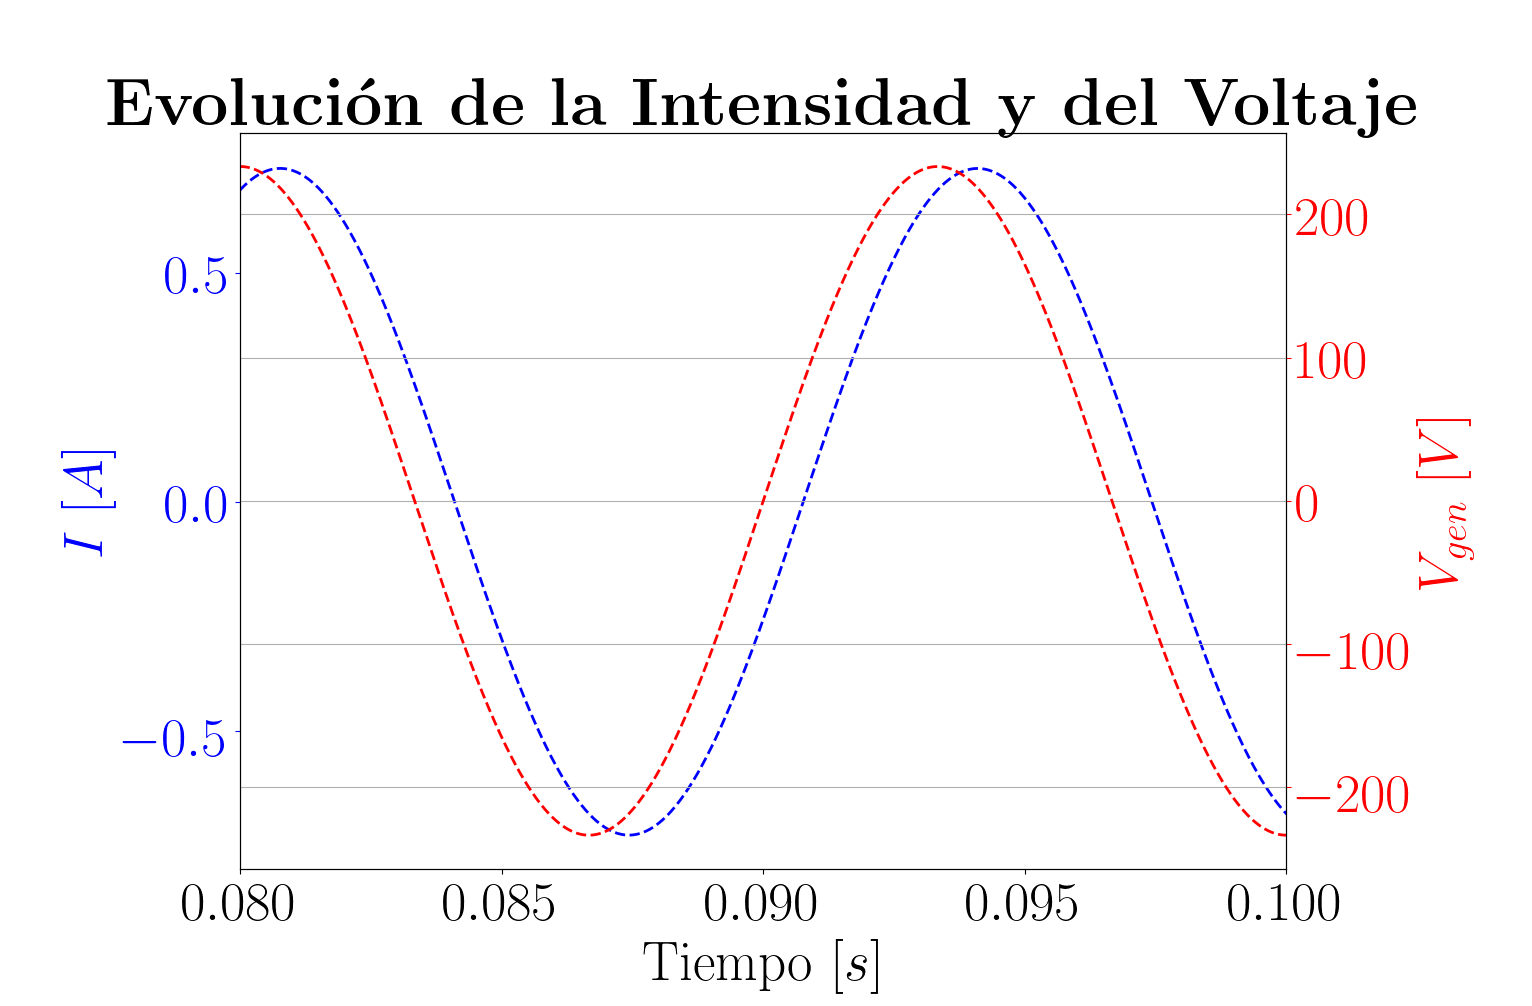
\includegraphics[width=\linewidth,trim={0 0 0 55},clip]{f75.png}
    \caption{Evolución de la intensidad y del voltaje para el circuito RLC con generador para una frecuencia $f = 75.00~[Hz]$.}
    \label{fig:f75}
\end{figure}

\newpage

\begin{figure}[!htb]
    \centering
    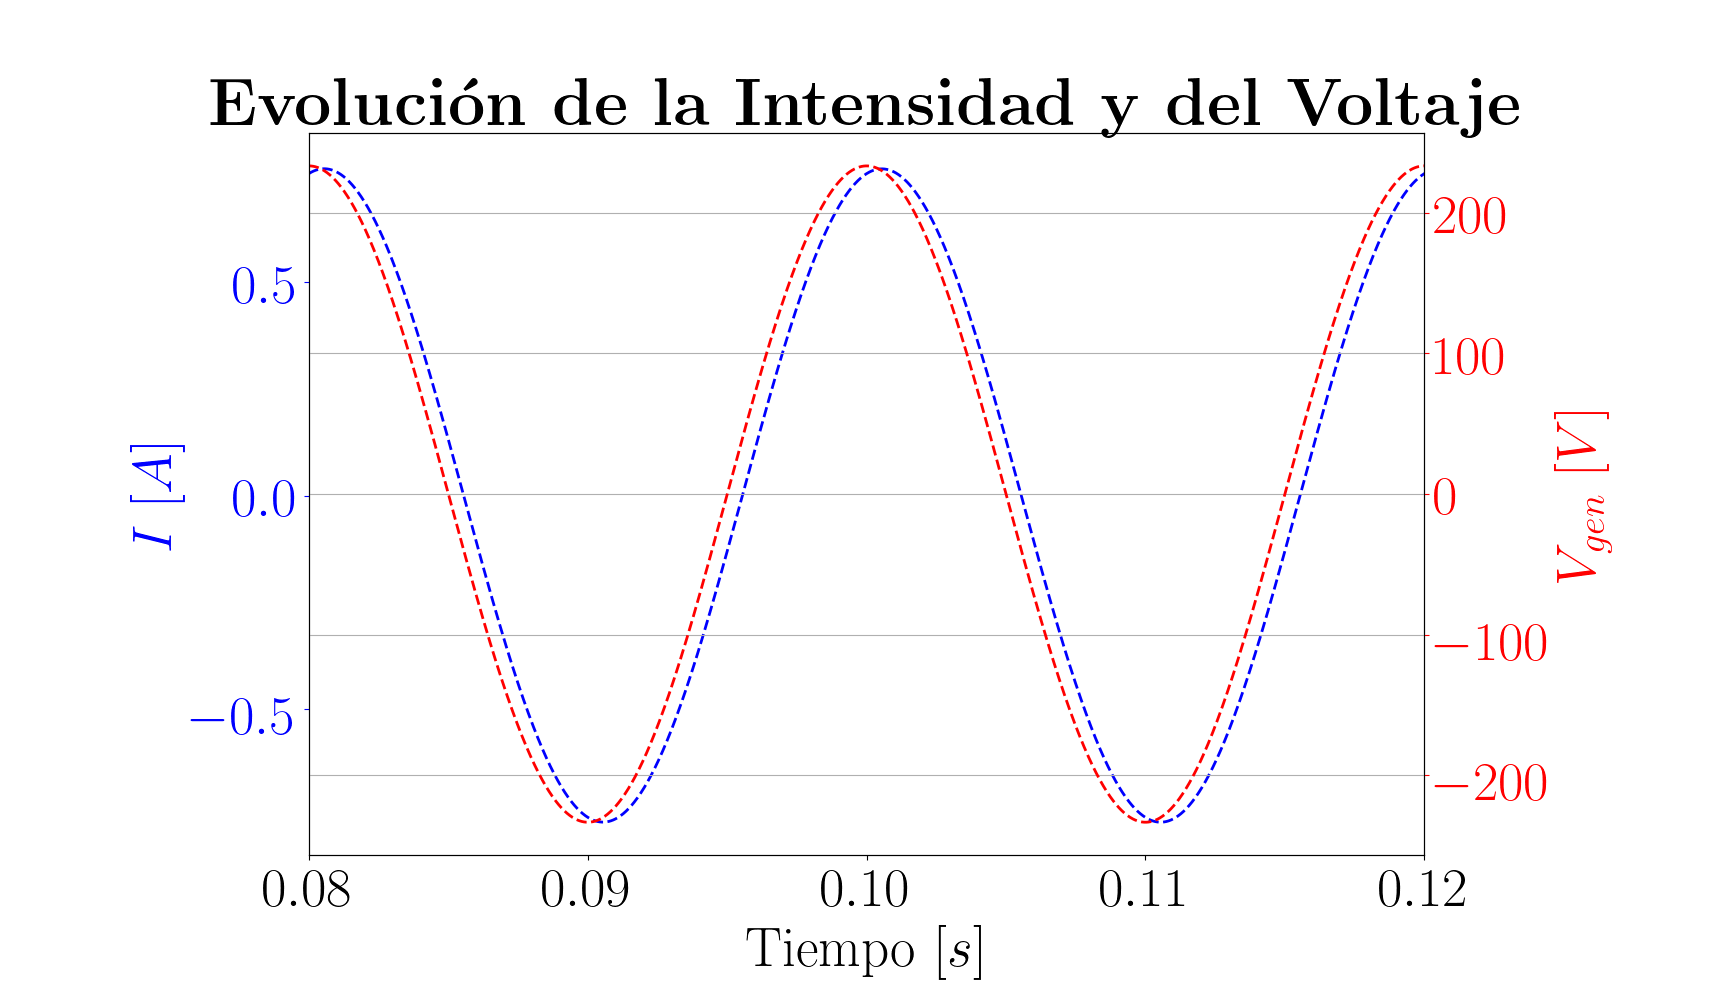
\includegraphics[width=\linewidth,trim={70 0 70 55},clip]{f50.png}
    \caption{Evolución de la intensidad y del voltaje para el circuito RLC con generador para una frecuencia $f = 50.00~[Hz]$.}
    \label{fig:f50}
\end{figure}

\begin{figure}[!htb]
    \centering
    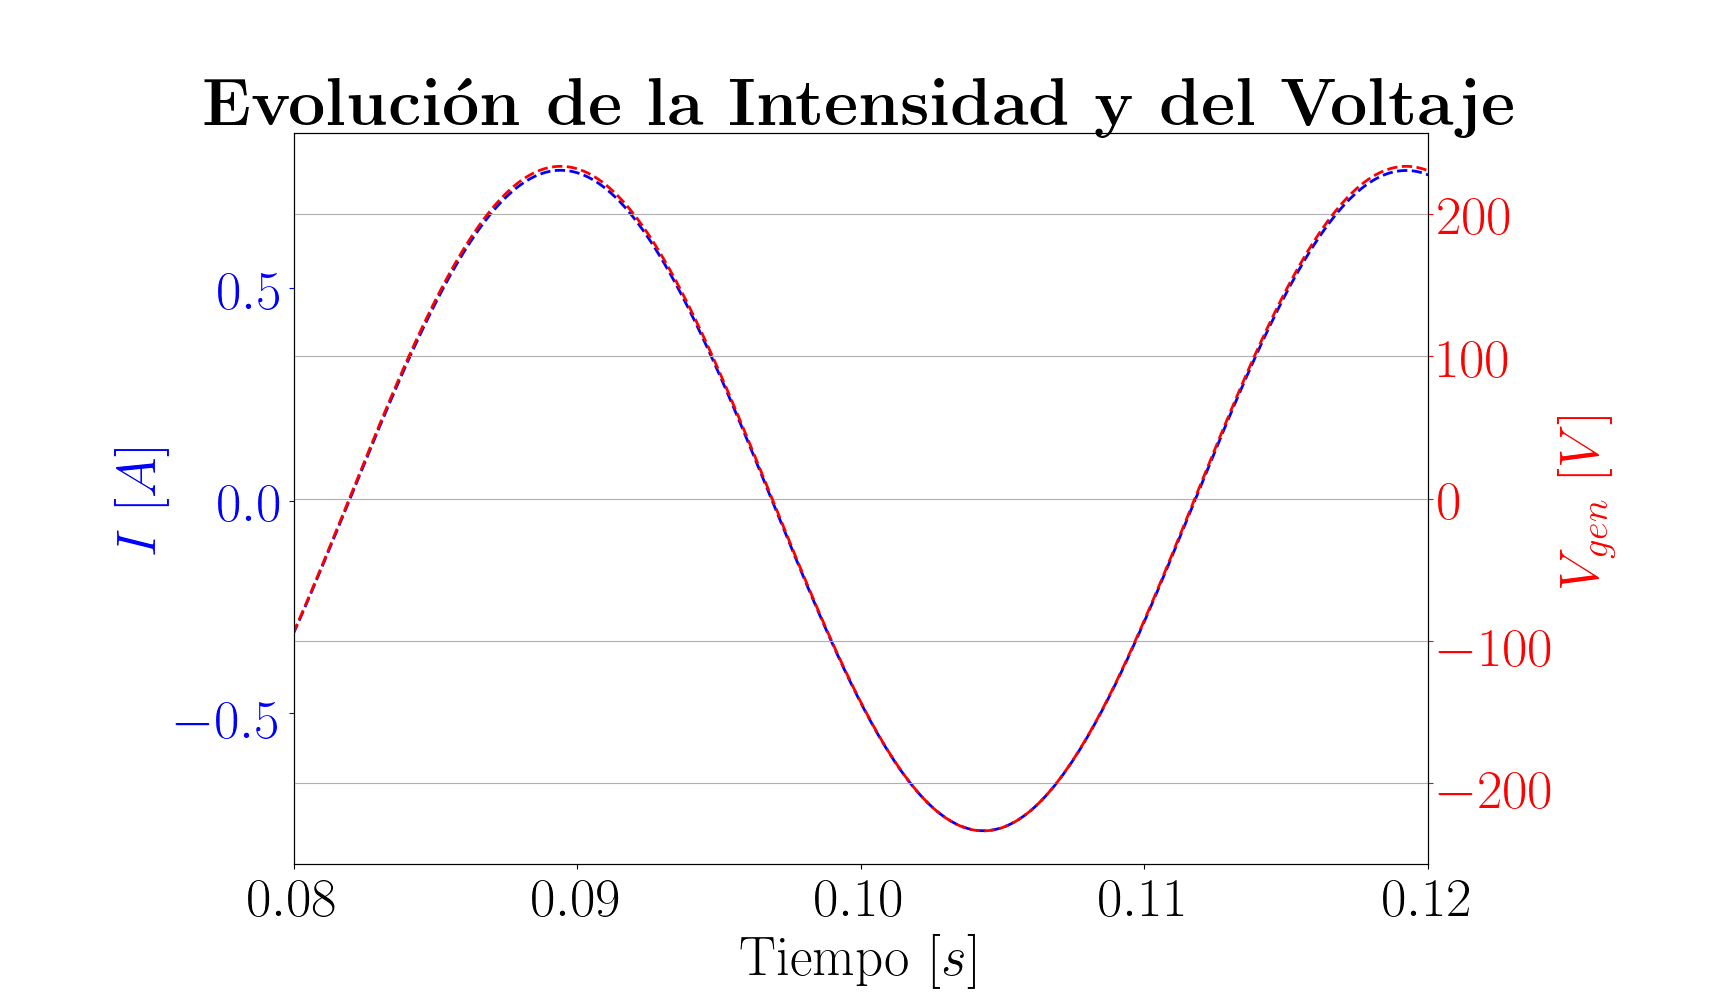
\includegraphics[width=\linewidth,trim={70 0 70 55},clip]{fres.png}
    \caption{Evolución de la intensidad y del voltaje para el circuito RLC con generador para una frecuencia $f = 33.55~[Hz]$ que coincide con la frecuencia de resonancia.}
    \label{fig:fres}
\end{figure}

\begin{figure}[!htb]
    \centering
    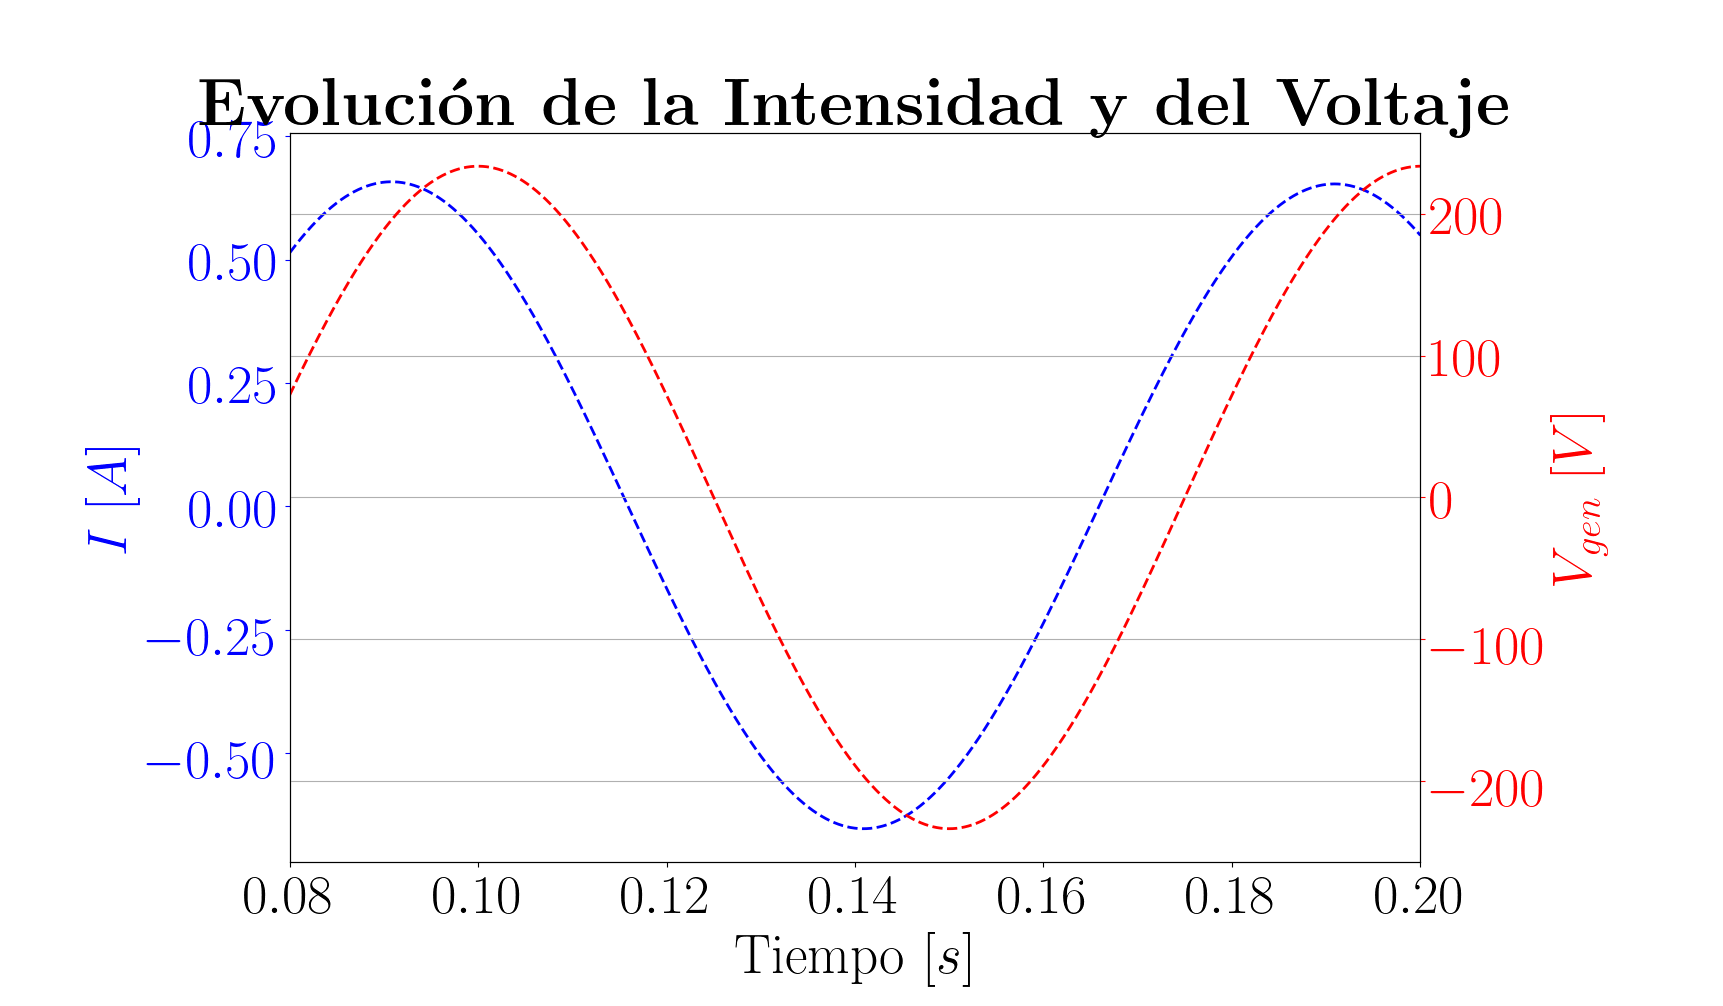
\includegraphics[width=\linewidth,trim={60 0 70 55},clip]{f10.png}
    \caption{Evolución de la intensidad y del voltaje para el circuito RLC con generador para una frecuencia $f = 10.00~[Hz]$.}
    \label{fig:f10}
\end{figure}

\newpage

\begin{figure}[!htb]
    \centering
    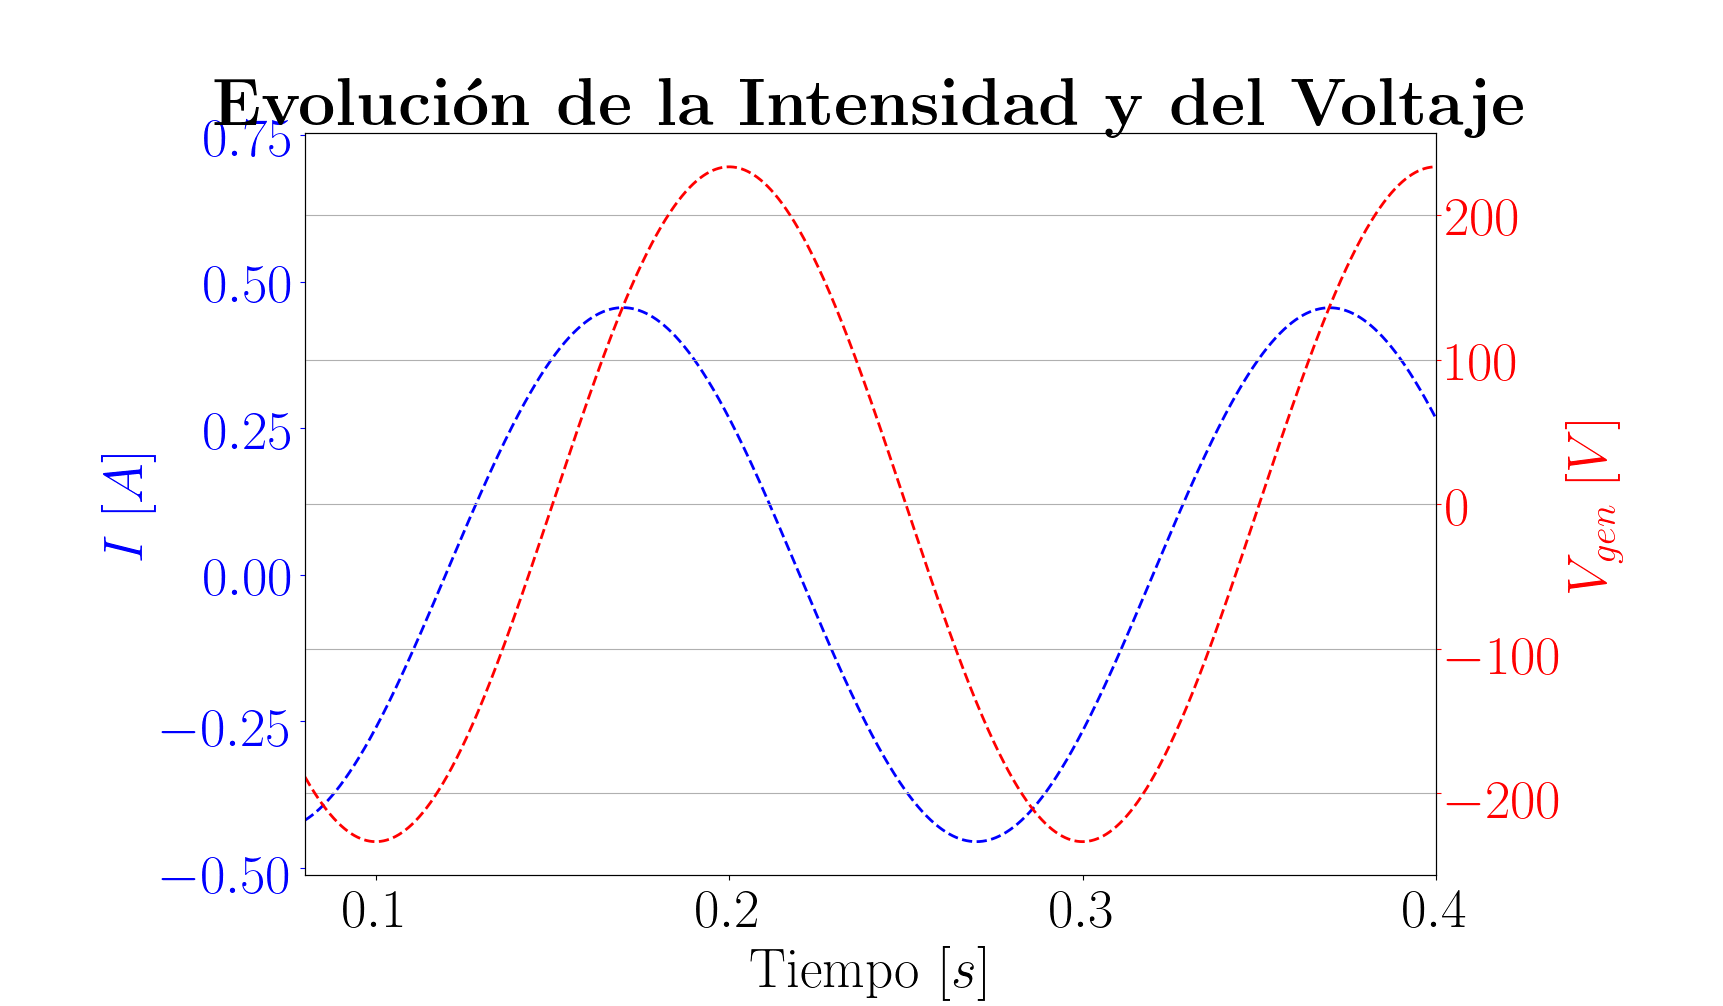
\includegraphics[width=\linewidth,trim={0 0 0 55},clip]{f5.png}
    \caption{Evolución de la intensidad y del voltaje para el circuito RLC con generador para una frecuencia $f = 5.00~[Hz]$.}
    \label{fig:f5}
\end{figure}

Como podemos comprobar, en el caso mostrado en la Figura \ref{fig:fres}, el desfase es nulo $\delta = 0~[rad]$ y el voltaje coincide con la intensidad a la vez que se obtiene la intensidad máxima de $I_0 \simeq 0.779~[A]$. La Figura \ref{fig:intensidadfrecuencia} muestra la evolución de la intensidad en función de la frecuencia elegida y viene a constatar que la intensidad máxima se alcanza cuando la frecuencia elegida se corresponde con la frecuencia de resonancia $f_{res}$. También mostramos los cálculos necesarios para obtener las diferentes intensidades:

\begin{equation}
I_0 = \frac{V_0}{Z} = \frac{V_0}{\sqrt{R^2 + (2\pi f L - \frac{1}{2\pi f C})^2}}
\end{equation}

\begin{equation}
I_{f=75} = \frac{165\sqrt{2}}{\sqrt{300^2 + (2\pi 75.00\cdot 0.30 - \frac{1}{2\pi 75.00\cdot 75.00\cdot 10^{-6}})^2}}
\end{equation}
\begin{equation}
I_{f=75} = 0.728~[A]
\end{equation}

\begin{equation}
I_{f=50} = \frac{165\sqrt{2}}{\sqrt{300^2 + (2\pi 50.00\cdot 0.30 - \frac{1}{2\pi 50.00\cdot 75.00\cdot 10^{-6}})^2}}
\end{equation}
\begin{equation}
I_{f=50} = 0.766~[A]
\end{equation}

\begin{equation}
I_{f=f_{res}} = \frac{165\sqrt{2}}{\sqrt{300^2 + (2\pi 33.55\cdot 0.30 - \frac{1}{2\pi 33.55\cdot 75.00\cdot 10^{-6}})^2}}
\end{equation}
\begin{equation}
I_{f=f_{res}} = 0.779~[A]
\end{equation}

\begin{equation}
I_{f=10} = \frac{165\sqrt{2}}{\sqrt{300^2 + (2\pi 10.00\cdot 0.30 - \frac{1}{2\pi 10.00\cdot 75.00\cdot 10^{-6}})^2}}
\end{equation}
\begin{equation}
I_{f=10} = 0.654~[A]
\end{equation}

\begin{equation}
I_{f=5} = \frac{165\sqrt{2}}{\sqrt{300^2 + (2\pi 5.00\cdot 0.30 - \frac{1}{2\pi 5.00\cdot 75.00\cdot 10^{-6}})^2}}
\end{equation}
\begin{equation}
I_{f=5} = 0.456~[A]
\end{equation}

\begin{figure}[!htb]
    \begin{tikzpicture}
        \begin{axis}[
            xlabel={$f = [Hz]$},
            ylabel={$I_0 = [A]$},
            xmin=0.0, xmax=80.0,
            ymin=0.0, ymax=1.0,
            enlargelimits=true,
            xtick={0.0, 10.0, 20.0, 30.0, 40.0, 50.0, 60.0, 70.0, 80.0},
            ytick={0.0, 0.1, 0.2, 0.3, 0.4, 0.5, 0.6, 0.7, 0.8, 0.9, 1.0},
            ymajorgrids=true,
            grid style=dashed,
        ]
         

        \addplot[
                smooth,
                color=red,
                mark=square,
                ]
                coordinates {
                    (5, 0.456)(10,0.654)(33.55,0.779)(50,0.766)(75,0.728)
                };
        \end{axis}
    \end{tikzpicture}
    \caption{Intensidad en función de la frecuencia.}
    \label{fig:intensidadfrecuencia}
\end{figure}

\section{Conclusión}
\label{sec:conclusion}

En esta segunda práctica de la asignatura hemos presentado sendos estudios sobre el comportamiento de circuitos RLC tanto en una situación de descarga de un condensador como en el caso de la aplicación de un generador de corriente alterna. En dichos estudios hemos sido capaces de analizar y comprender la evolución de su dinámica: de la intensidad que circula por el circuito, del voltaje existente y de la energía tanto almacenada como disipada.

Gracias a la realización de esta práctica y de su informe hemos consolidado en gran medida el conocimiento sobre circuitos RLC y de corriente alterna.

El código Python que implementa esta práctica así como las fuentes \LaTeX de este informe se encuentran disponibles online en el repositorio \url{https://github.com/Blitzman/physics/tree/master/fisica_2/practica_2}.


\end{document}
